% last updated in April 2002 by Antje Endemann
% Based on CVPR 07 and LNCS, with modifications by DAF, AZ and elle, 2008 and AA, 2010, and CC, 2011; TT, 2014

\documentclass[runningheads]{llncs}
\usepackage{graphicx}
\usepackage{amsmath,amssymb} % define this before the line numbering.
\usepackage{ruler}
\usepackage{color}
\usepackage{subfigure}
\usepackage[width=122mm,left=12mm,paperwidth=146mm,height=193mm,top=12mm,paperheight=217mm]{geometry}
%\usepackage{tikz}
\usepackage[percent]{overpic}
\begin{document}
% \renewcommand\thelinenumber{\color[rgb]{0.2,0.5,0.8}\normalfont\sffamily\scriptsize\arabic{linenumber}\color[rgb]{0,0,0}}
% \renewcommand\makeLineNumber {\hss\thelinenumber\ \hspace{6mm} \rlap{\hskip\textwidth\ \hspace{6.5mm}\thelinenumber}}
% \linenumbers
\pagestyle{headings}
\mainmatter
\def\ECCV14SubNumber{***}  % Insert your submission number here

\title{Beyond the Google StreetView: learning predictors for architecture stlye, graffiti and vegetation } % Replace with your title

\titlerunning{ECCV-14 submission ID \ECCV14SubNumber}

\authorrunning{ECCV-14 submission ID \ECCV14SubNumber}

\author{Anonymous ECCV submission}
\institute{Paper ID \ECCV14SubNumber}


\maketitle

\begin{abstract}
  Given a large database of geotagged imagery of a whole city the goal is to evaluate a distribution of different architecture styles across the city and to detect areas with high occurance of graffiti. We also aim on detecting areas with open or close view or areas with dense or loose vegetation. We first download 180,000 panoramas of the city of Madrid from the Google street view, then we generate a random set of 7,000 perspective images and label them. We use the labeled images to train a set of linear SVM predictors for each class. Finally, we uniformly sample 120,000 random images across the city of Madrid covering roughly area of $32 \times 36km$ and generate a set of heatmaps showing response of the learned predictors for different classes. The contribution of the paper is two fold: (i) We propose a simple method for detection of architecture style, graffiti, vegetation and view. We show that response of the classifier is semanticly correct. (ii) We have created a labeled set of images that is going to be publicly available.
  \keywords{We would like to encourage you to list your keywords within the abstract section}
\end{abstract}


\section{Introduction}

\section{Related work}

\section{Approach overview}

% \begin{tikzpicture}
%     \node[anchor=south west,inner sep=0] at (0,0) {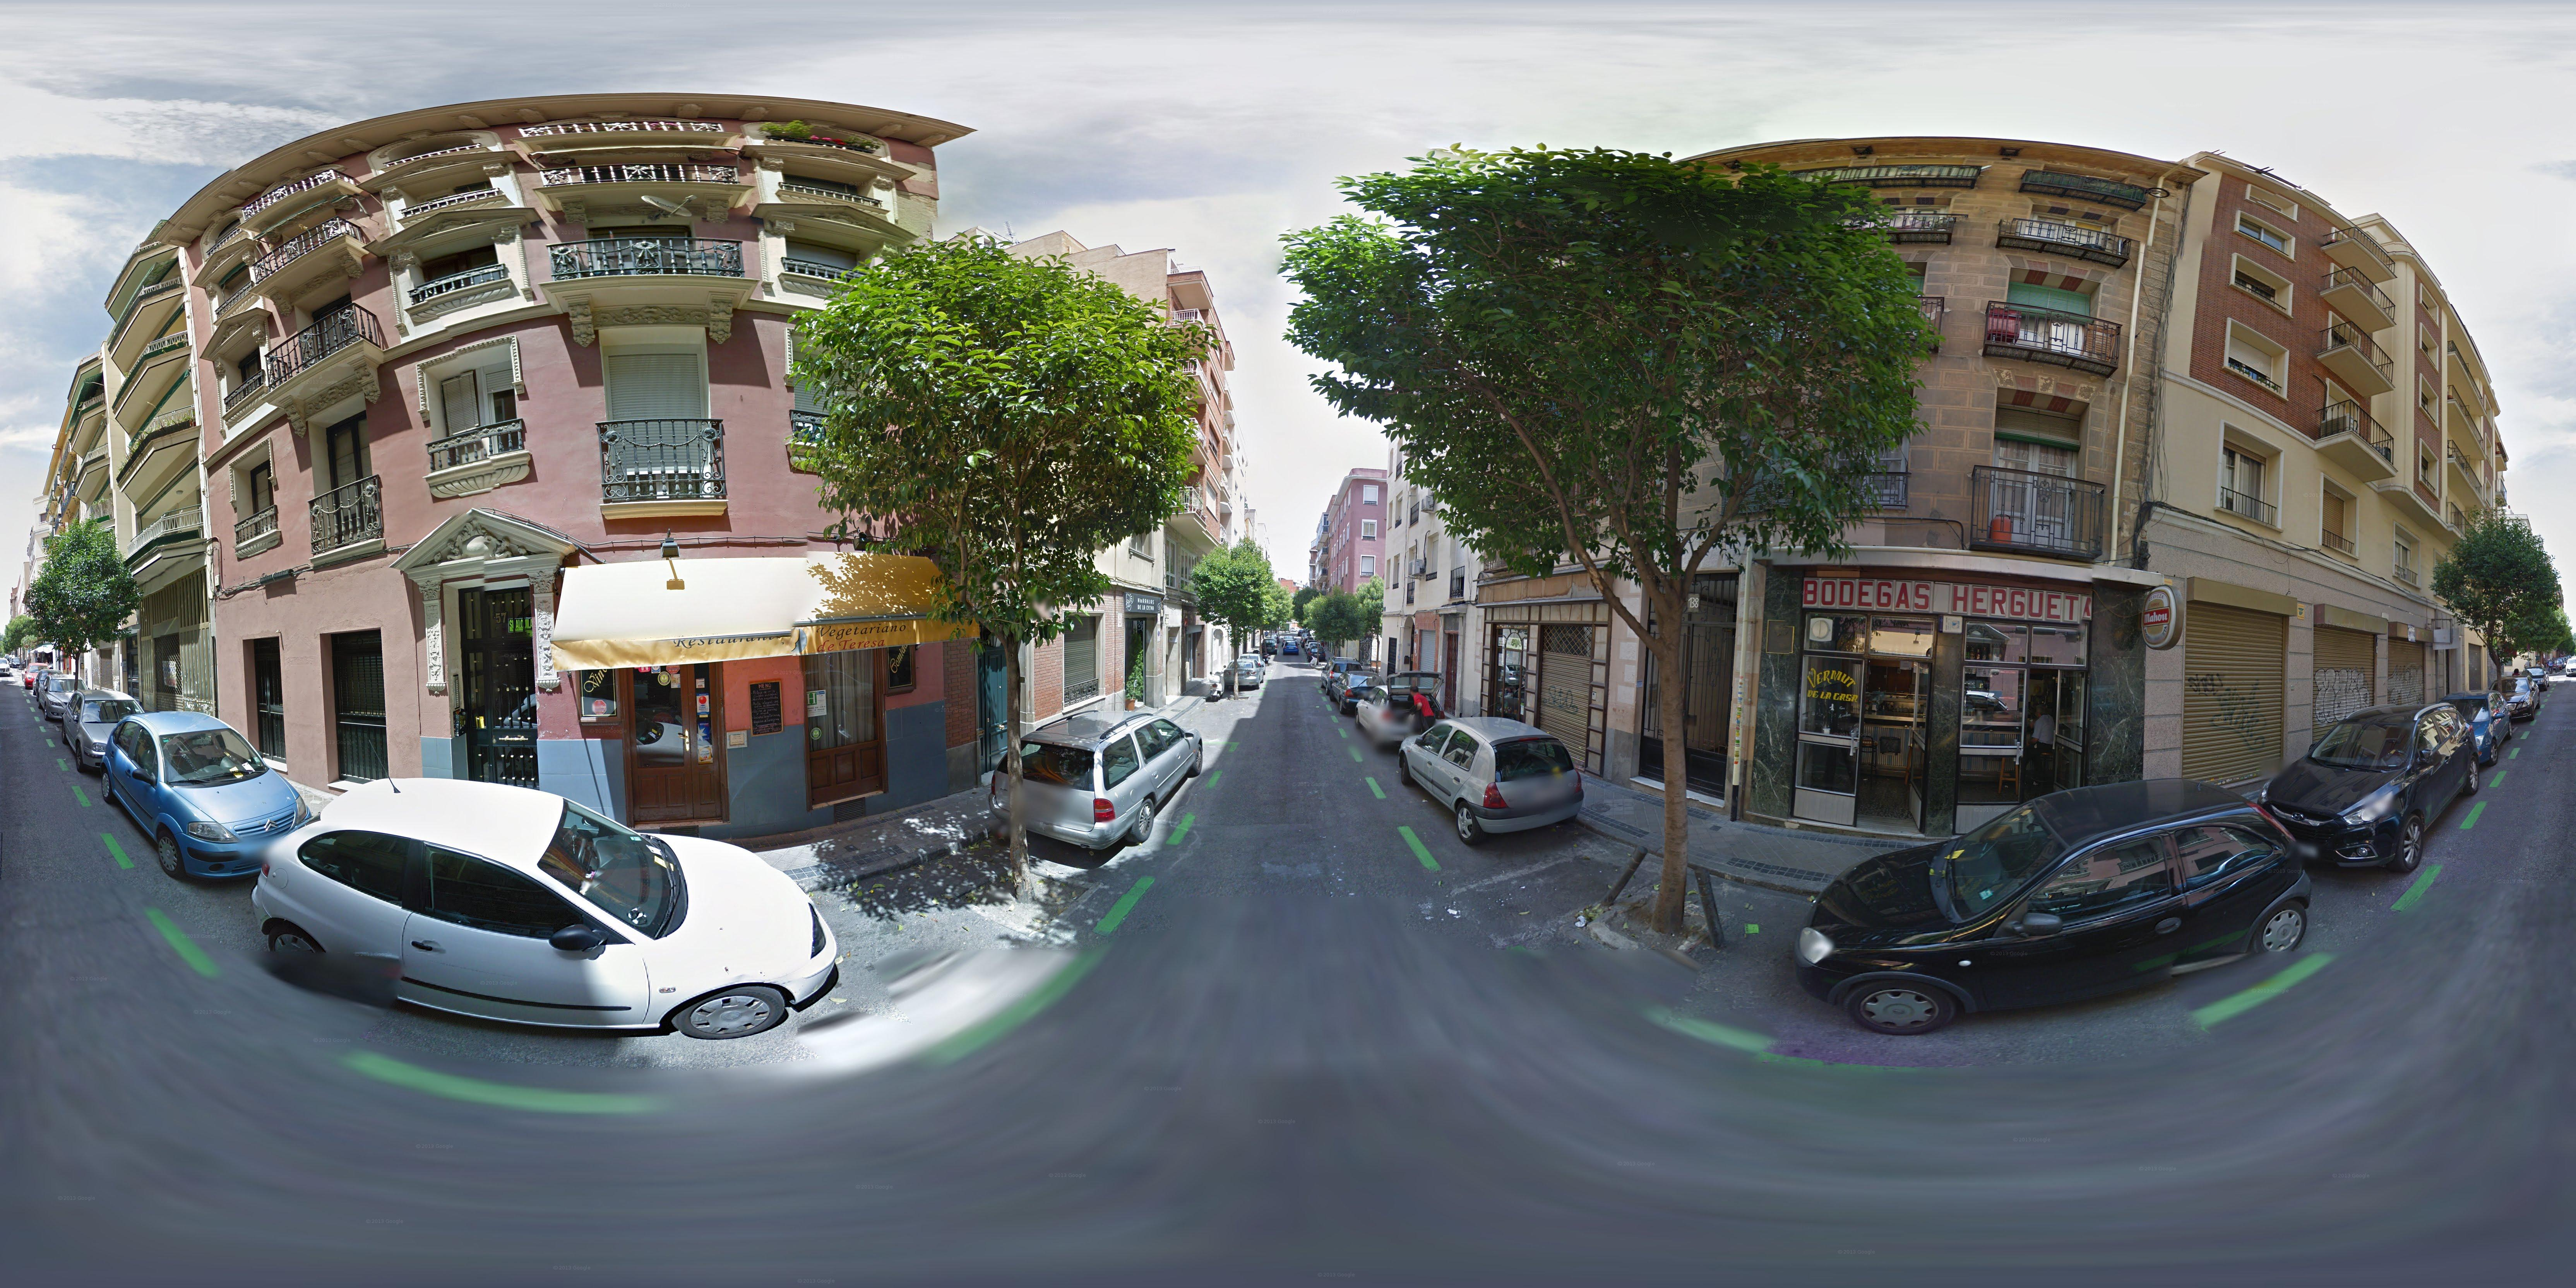
\includegraphics[width=\textwidth]{imgs/panorama}};
%     \draw[red,ultra thick,rounded corners] (7.5,5.3) rectangle (9.4,6.2);
% \end{tikzpicture}

% \begin{figure}
%   %\includegraphics[width=\linewidth]{}
%   \caption{}
%   \label{}
% \end{figure}

%%% Image: Google panorama
\begin{figure}[t]
  \begin{minipage}{0.3\linewidth}
    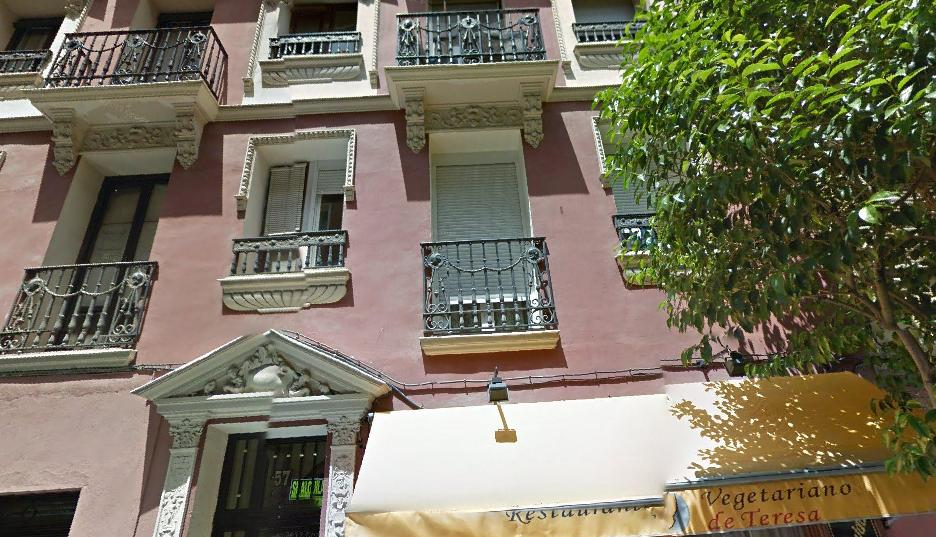
\includegraphics[width=\linewidth]{imgs/cutout_pitch28.jpg} \\ \vspace{-3.5mm} \\
    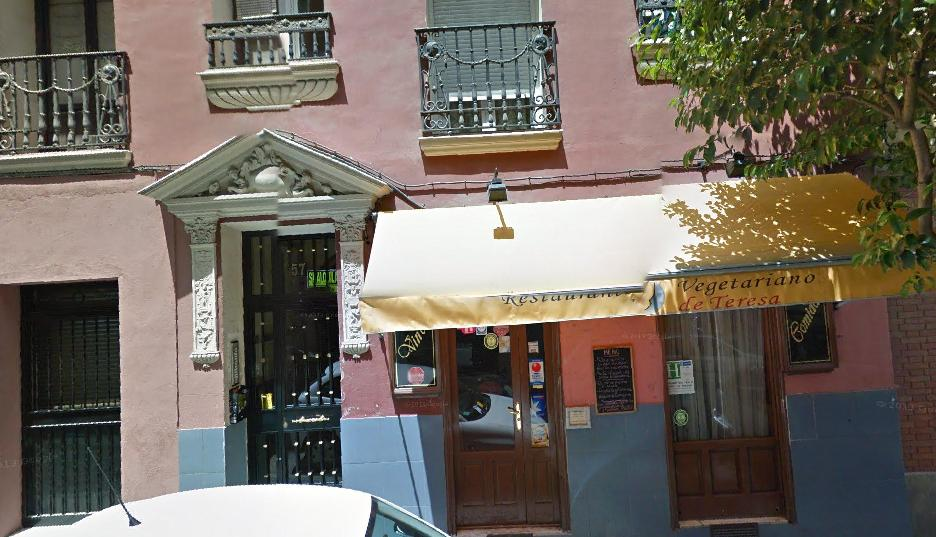
\includegraphics[width=\linewidth]{imgs/cutout_pitch04.jpg}
  \end{minipage}
  \begin{minipage}{0.7\linewidth}
    \begin{overpic}[width=\textwidth]{imgs/panorama.jpg}
      %%% Lines
      \linethickness{0.15mm}
        \put(50,0){\color{blue}\vector(0,1){50}}  %center line
      {\color{red}
        \put(25,0){\color{red}\vector(0,1){50}}   % left line
        \put(75,0){\color{red}\vector(0,1){50}}   % right line
        \multiput(12.5,-6)(0,2){28}                    % FOV left
          {\line(0,1){1}}
        \multiput(37.5,-6)(0,2){28}                    % FOV right
          {\line(0,1){1}} 
        \put(12.5,-4.5){\vector(1,0){25}}
        \put(37.5,-4.5){\vector(-1,0){25}}
      }
      %%% Text
      \put(21,-8){\color{black} \scriptsize FOV $90^\circ$}
      \put(47,-3){\color{black} \scriptsize Google}
      \put(44,-6){\color{black} \scriptsize car direction}
      \put(21,-3){\color{black} \scriptsize left side}
      \put(71,-3){\color{black} \scriptsize right side}
    \end{overpic}
  \end{minipage}
  \vspace{5mm}
  \caption{
  A center of each panorama \emph{(right)} corresponds to the Google car motion. For each side of the panorama we generate two perspective images \emph{(left)} with horizontal field of view $90^\circ$ in two different elevation pitches in order to capture both street view level and building facades.
  }
\end{figure}

%%% Image: Architecture
\begin{figure}
  \begin{minipage}{\linewidth}
    \begin{minipage}{0.3\linewidth}
      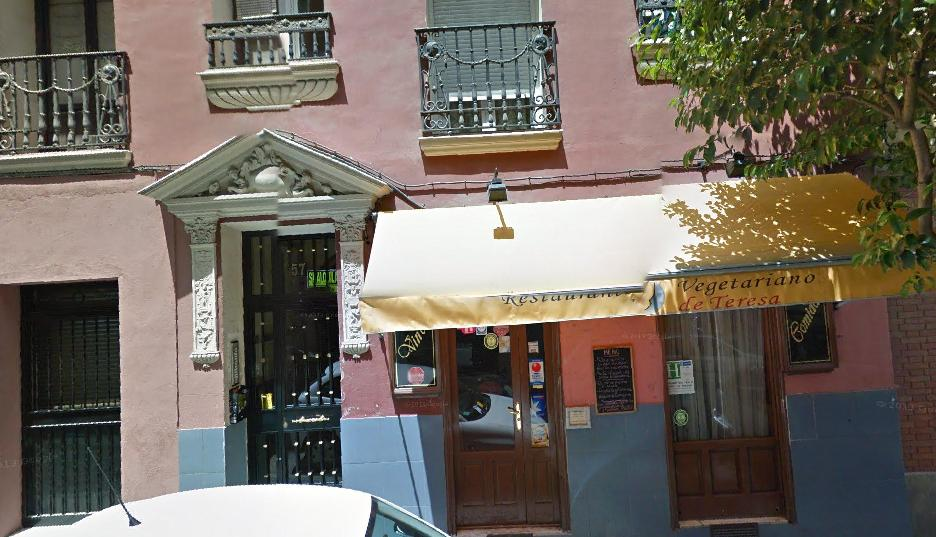
\includegraphics[width=0.49\linewidth]{imgs/cutout_pitch04.jpg}
      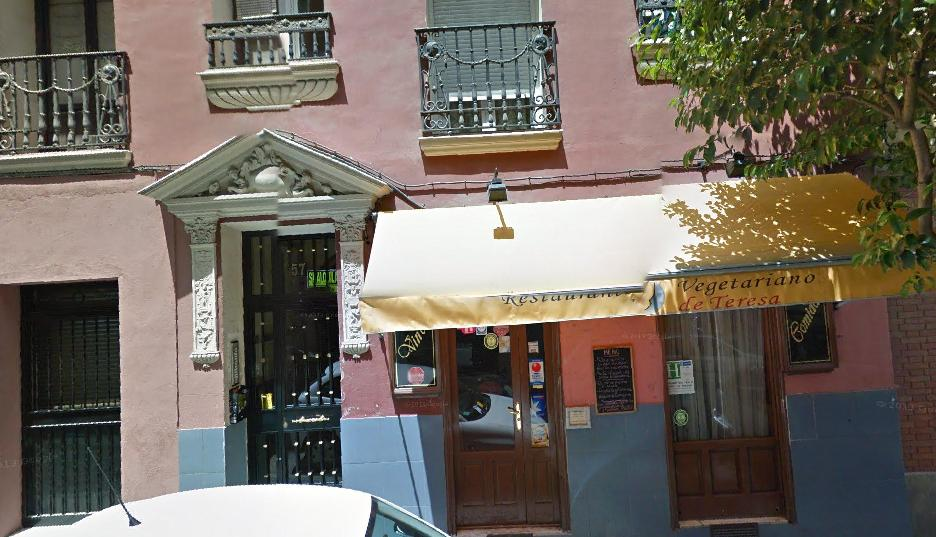
\includegraphics[width=0.49\linewidth]{imgs/cutout_pitch04.jpg}
      \\ \vspace{-3mm} \\
      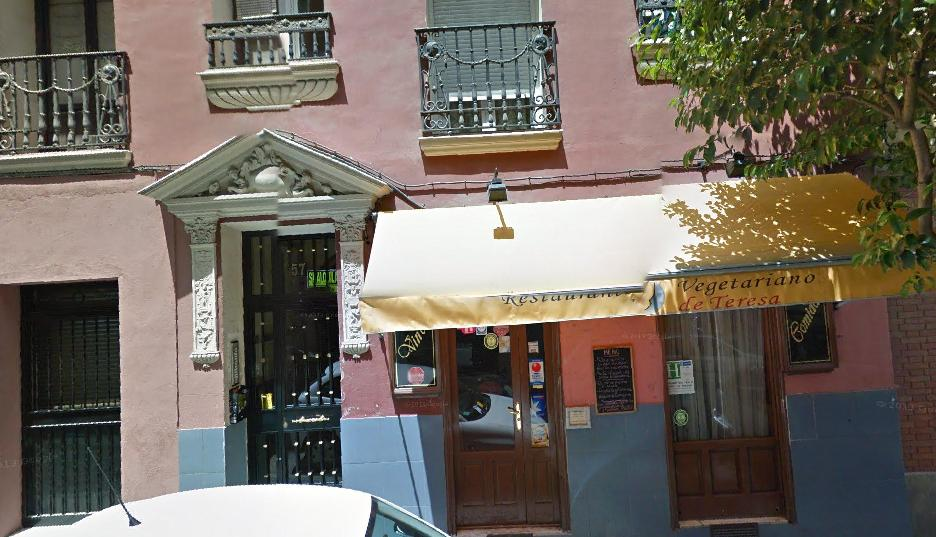
\includegraphics[width=0.49\linewidth]{imgs/cutout_pitch04.jpg}
      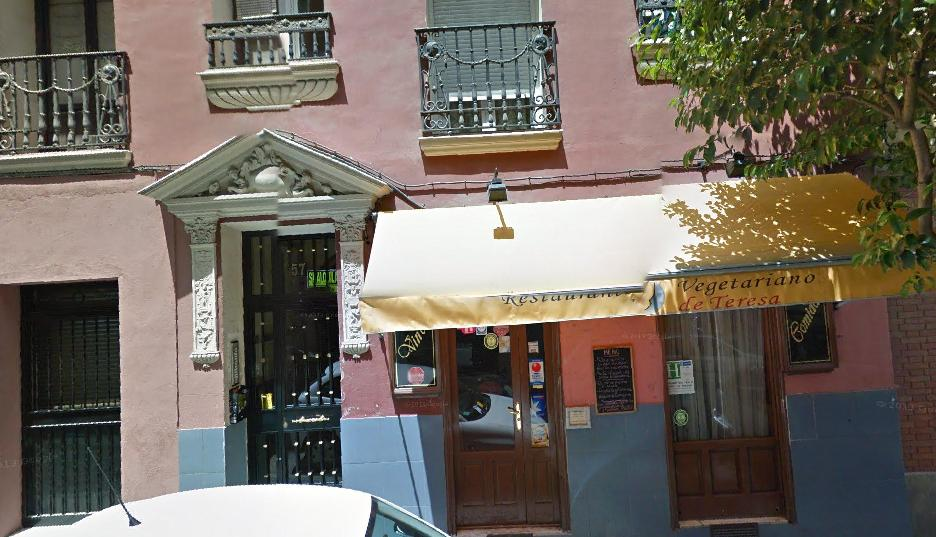
\includegraphics[width=0.49\linewidth]{imgs/cutout_pitch04.jpg}
      \\ \vspace{-3mm} \\
      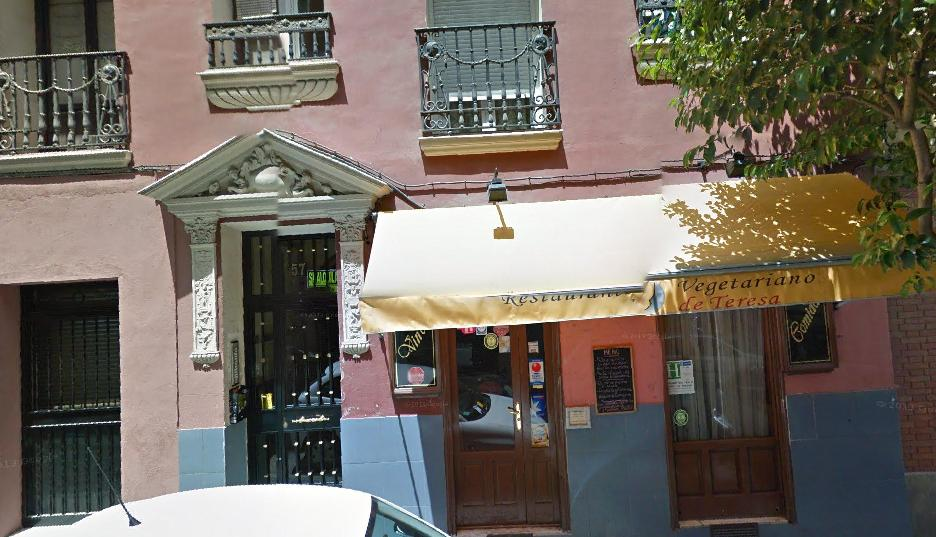
\includegraphics[width=0.49\linewidth]{imgs/cutout_pitch04.jpg}
      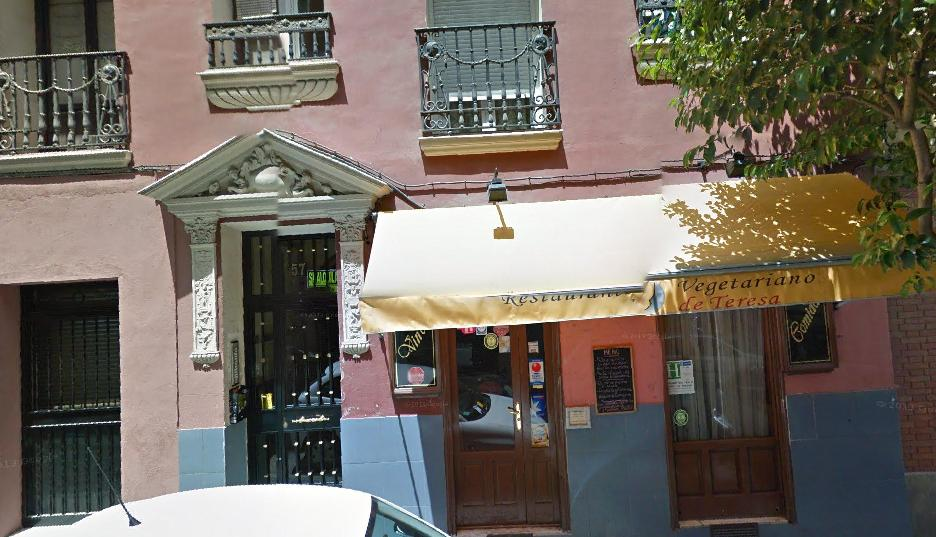
\includegraphics[width=0.49\linewidth]{imgs/cutout_pitch04.jpg}
      \\ \vspace{-3mm} \\
      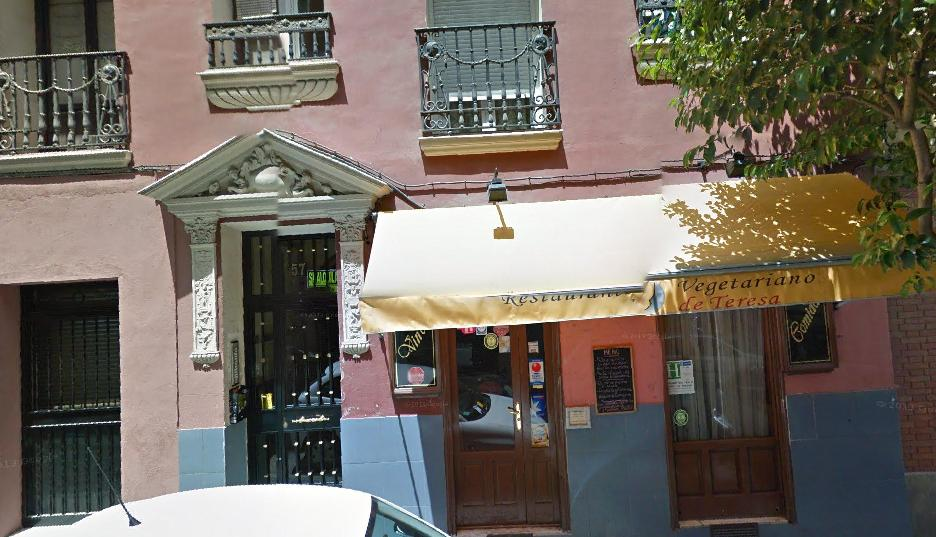
\includegraphics[width=0.49\linewidth]{imgs/cutout_pitch04.jpg}
      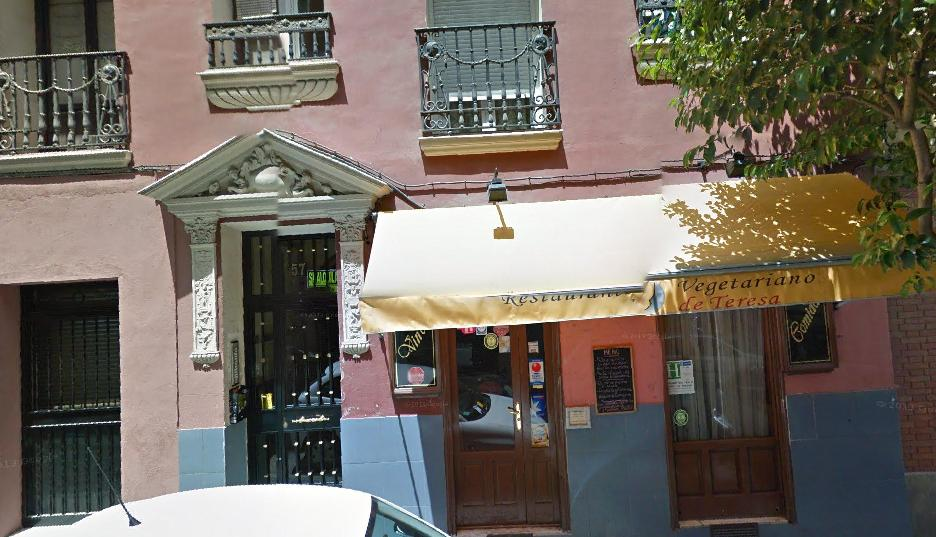
\includegraphics[width=0.49\linewidth]{imgs/cutout_pitch04.jpg}
      \\ \vspace{-3mm} \\
      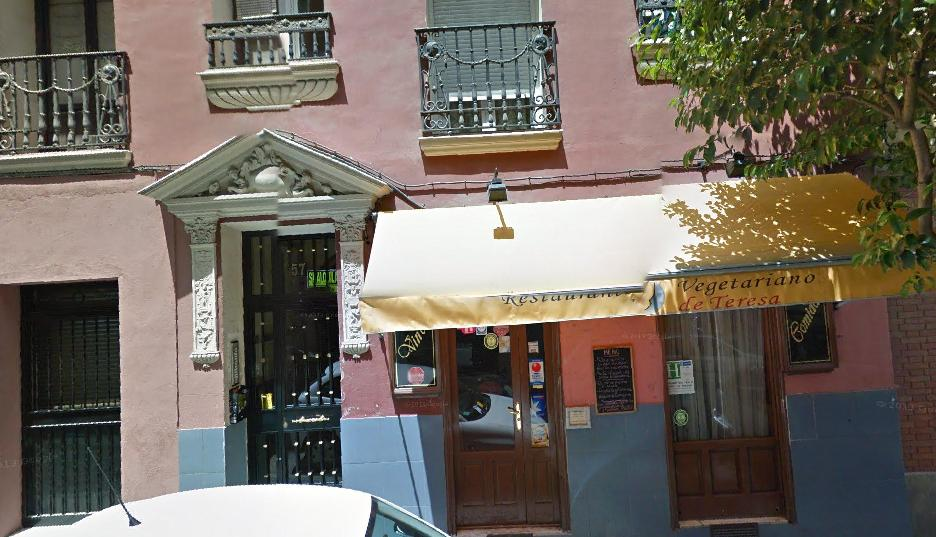
\includegraphics[width=0.49\linewidth]{imgs/cutout_pitch04.jpg}
      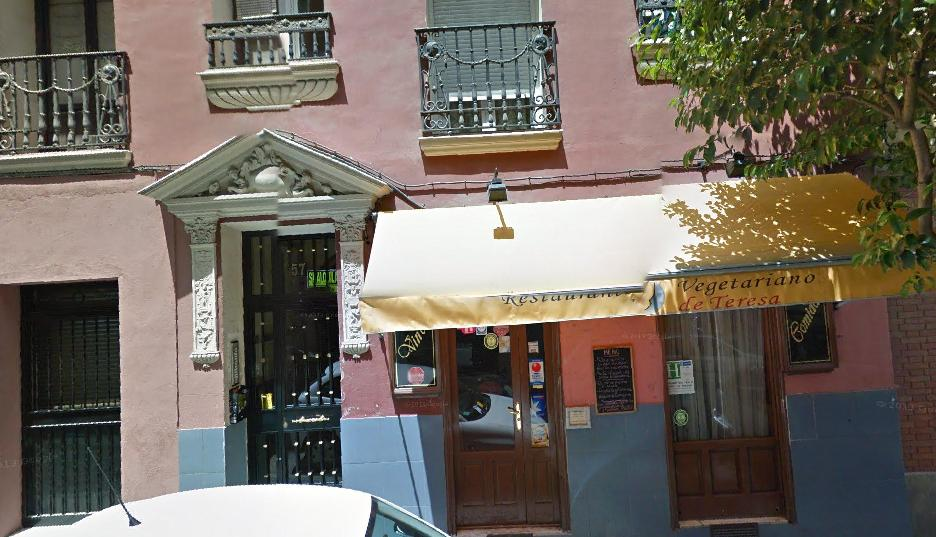
\includegraphics[width=0.49\linewidth]{imgs/cutout_pitch04.jpg}
    \end{minipage}
    \begin{minipage}{0.7\linewidth}
      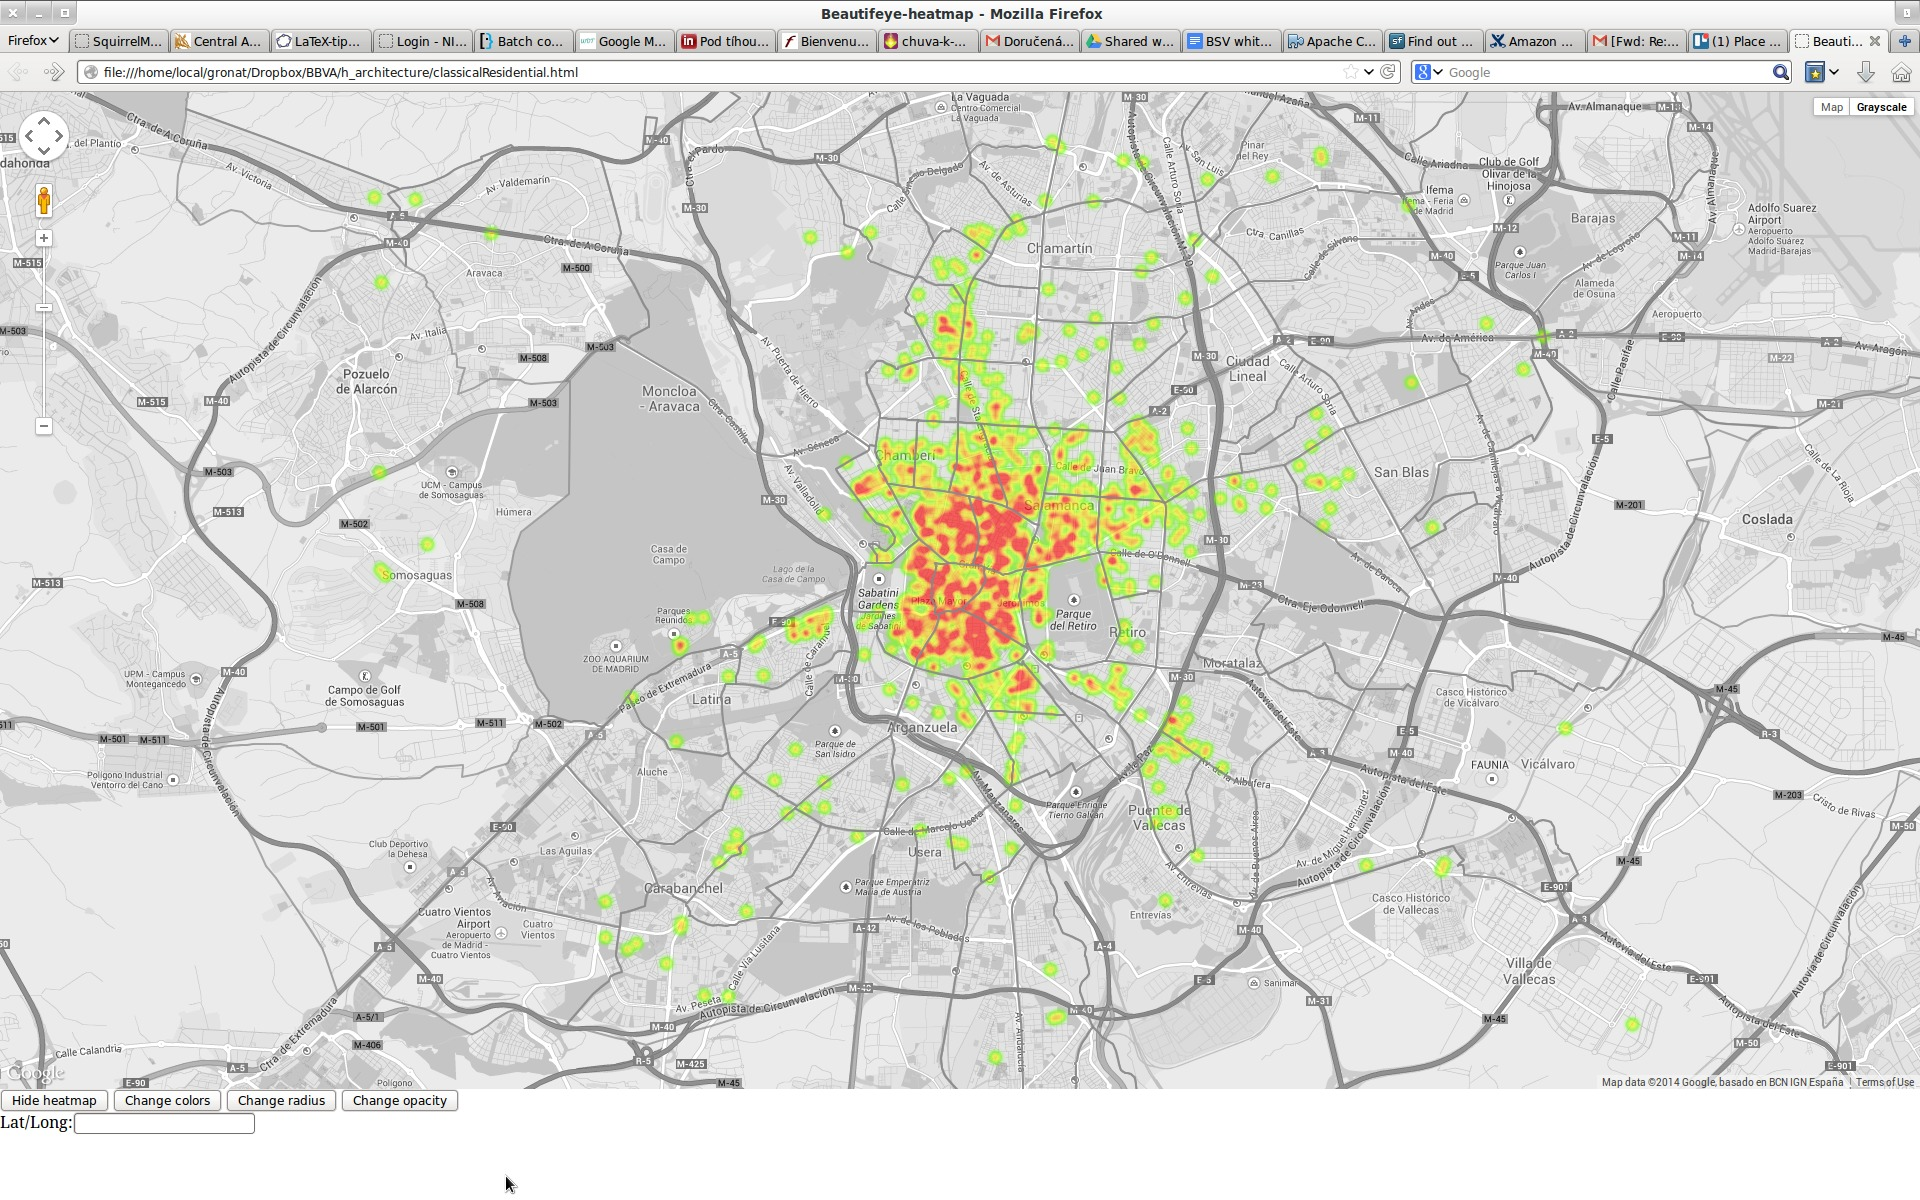
\includegraphics[trim= 350 150 250 150, clip=true, width=\linewidth]{imgs/arch/mapS2.jpg}
    \end{minipage}
  \end{minipage}
  \\
  $\;$ \hspace{30mm} (a) Classical residential
  \\
  \\
  \begin{minipage}{\linewidth}
    \begin{minipage}{0.3\linewidth}
      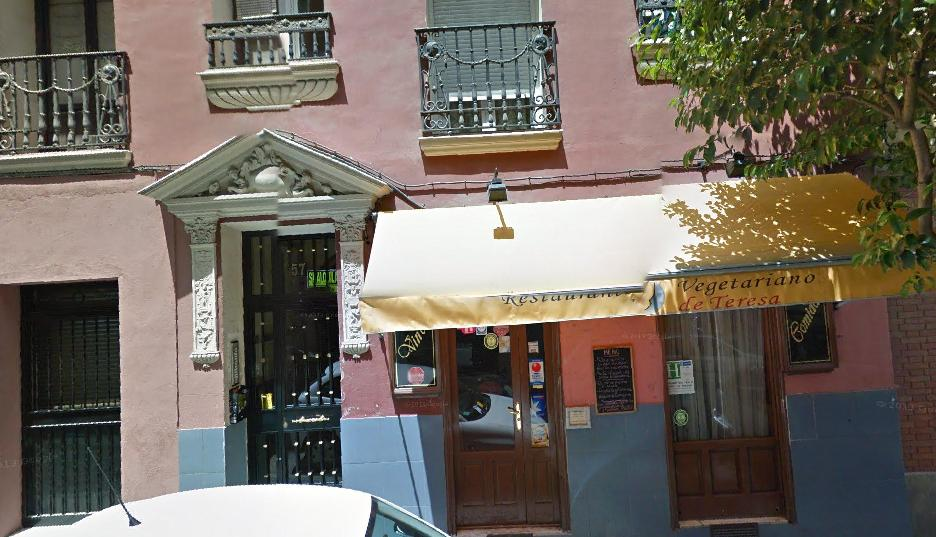
\includegraphics[width=0.49\linewidth]{imgs/cutout_pitch04.jpg}
      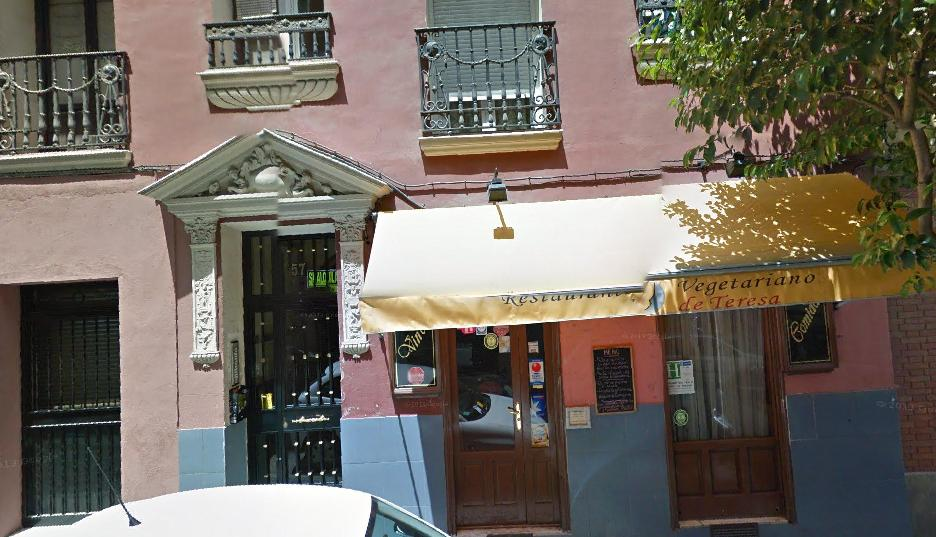
\includegraphics[width=0.49\linewidth]{imgs/cutout_pitch04.jpg}
      \\ \vspace{-3mm} \\
      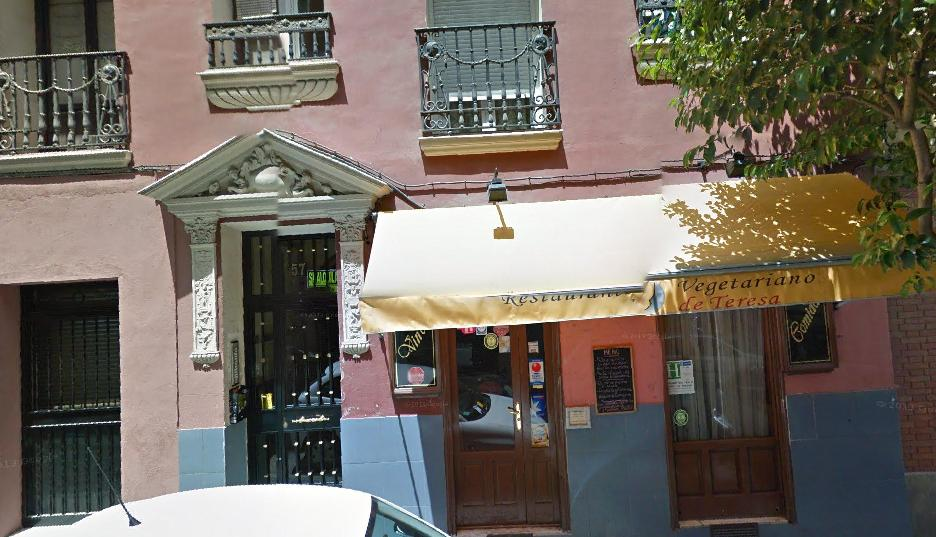
\includegraphics[width=0.49\linewidth]{imgs/cutout_pitch04.jpg}
      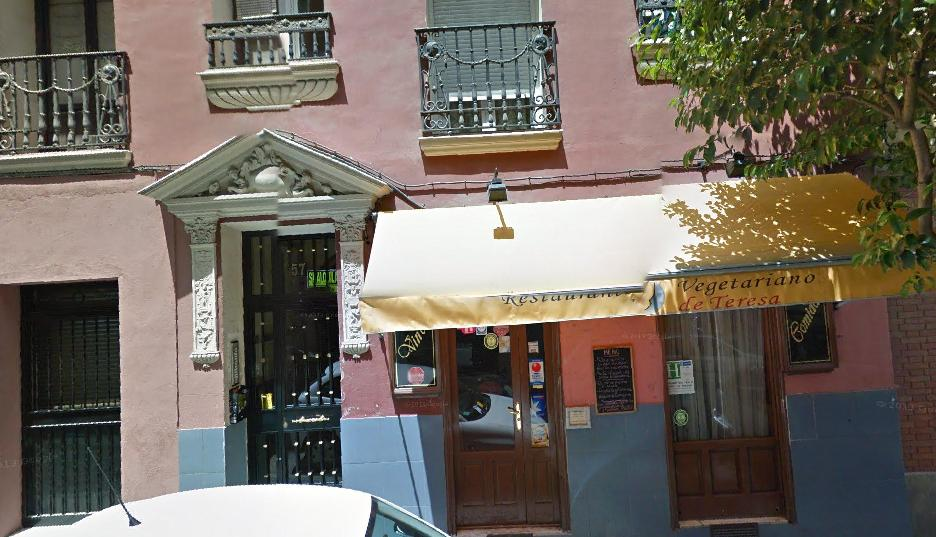
\includegraphics[width=0.49\linewidth]{imgs/cutout_pitch04.jpg}
      \\ \vspace{-3mm} \\
      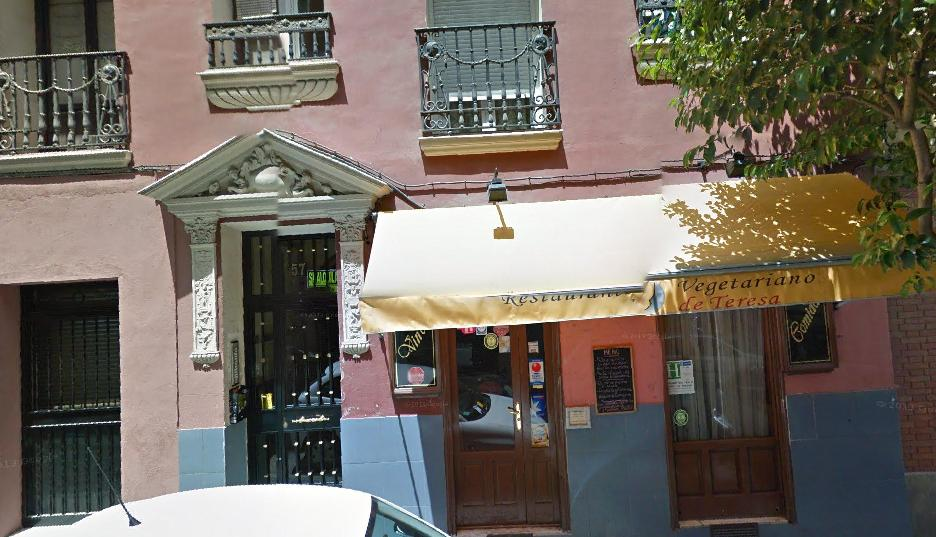
\includegraphics[width=0.49\linewidth]{imgs/cutout_pitch04.jpg}
      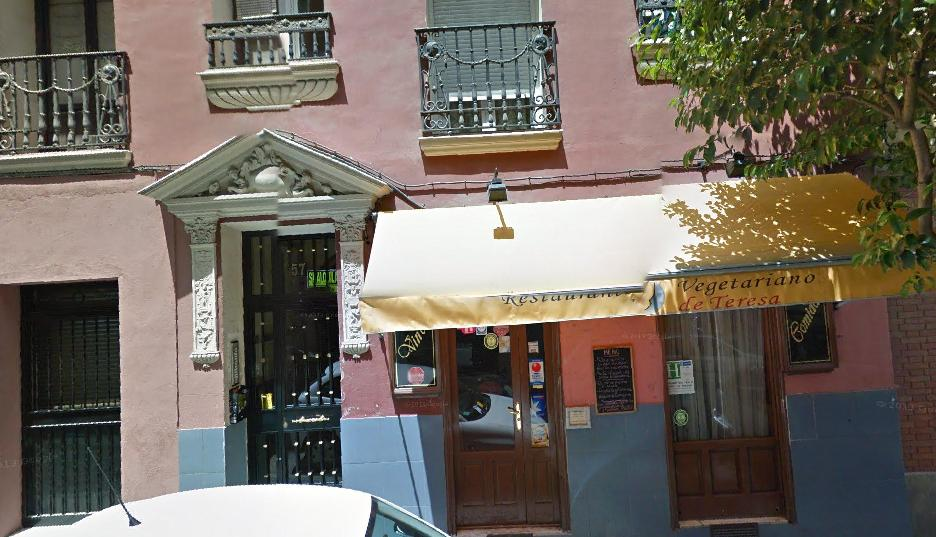
\includegraphics[width=0.49\linewidth]{imgs/cutout_pitch04.jpg}
      \\ \vspace{-3mm} \\
      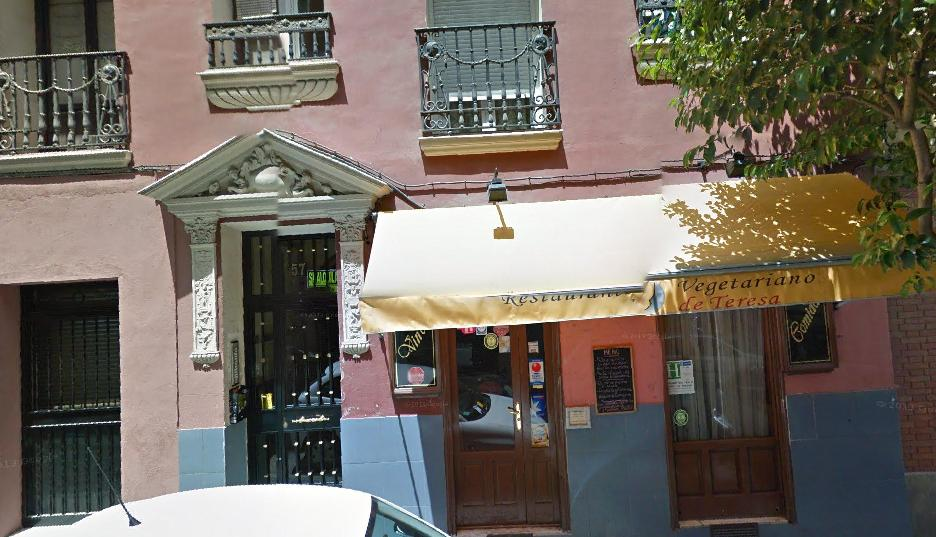
\includegraphics[width=0.49\linewidth]{imgs/cutout_pitch04.jpg}
      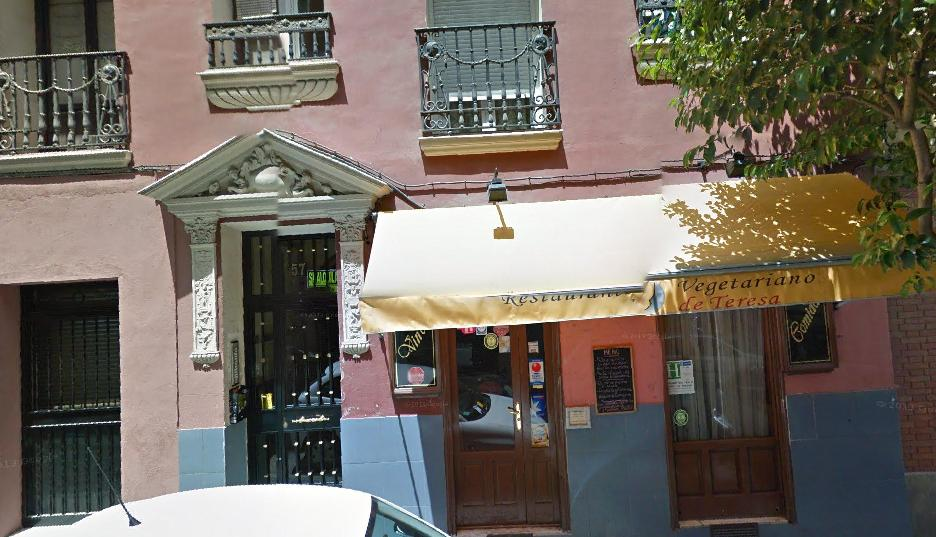
\includegraphics[width=0.49\linewidth]{imgs/cutout_pitch04.jpg}
      \\ \vspace{-3mm} \\
      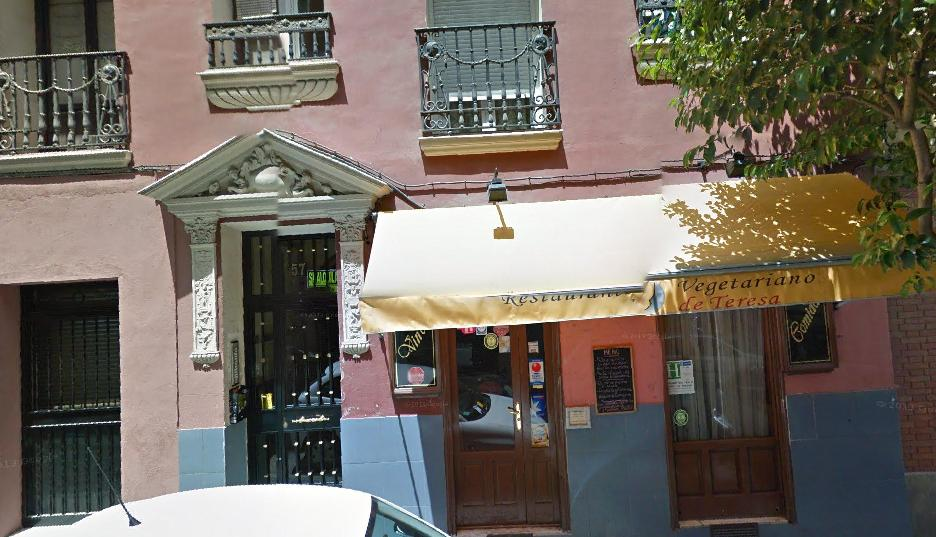
\includegraphics[width=0.49\linewidth]{imgs/cutout_pitch04.jpg}
      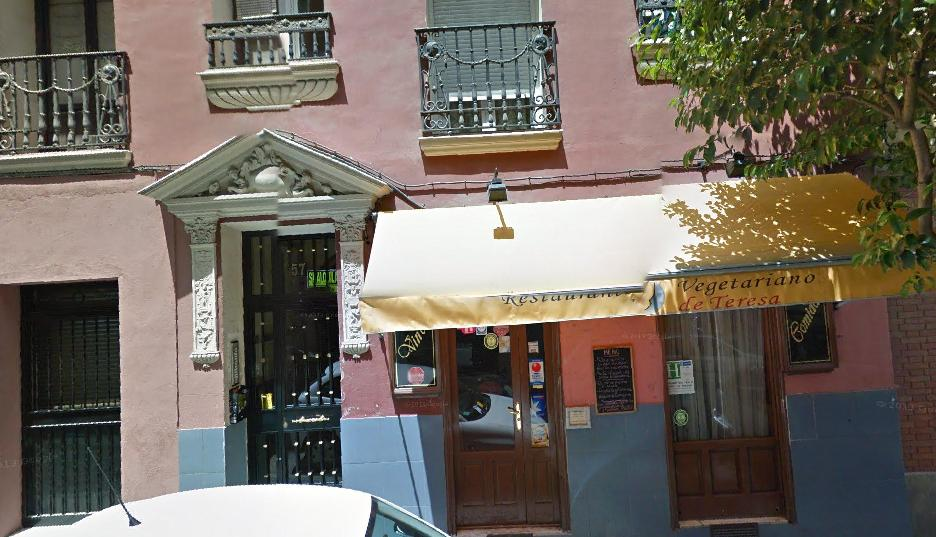
\includegraphics[width=0.49\linewidth]{imgs/cutout_pitch04.jpg}
    \end{minipage}
    \begin{minipage}{0.7\linewidth}
      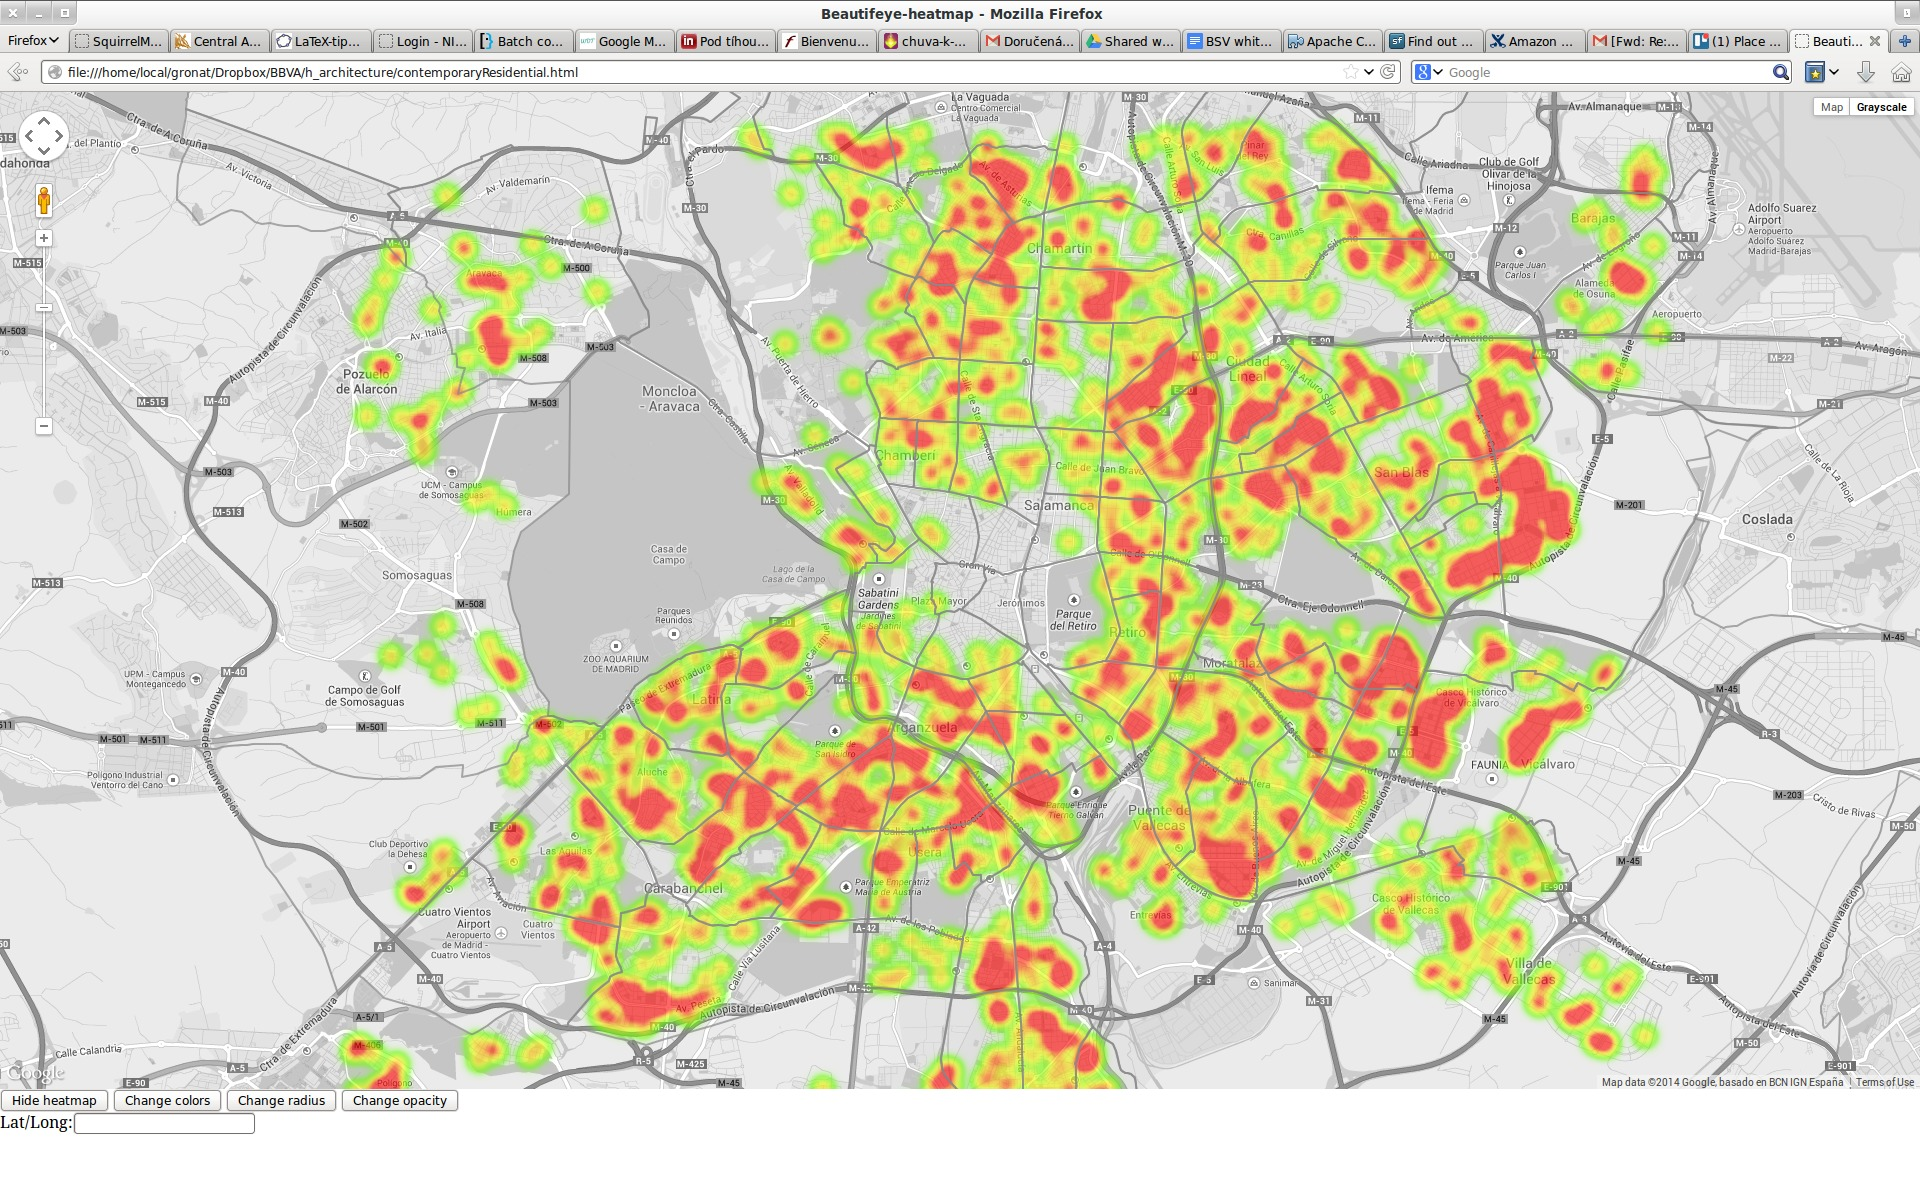
\includegraphics[trim= 350 150 250 150, clip=true, width=\linewidth]{imgs/arch/mapS3.jpg}
    \end{minipage}
  \end{minipage}
  \\
  $\;$\hspace{30mm} (b) Contemporary residential
  \\
  \caption{
    Architecture style: Heatmaps \emph{(right)} showing a density of different architecture styles across the city of Madrid. Notice that while \emph{classical residential} style (a) is mostly concentrated in the city center the \emph{contemporary residential} style (b) is detected away from the city center. On the \emph{left} there are examples of several top-ranked images for given style.
  }
\end{figure}


%%% Image: Vegetation
\begin{figure}
  \begin{minipage}{\linewidth}
    \begin{minipage}{0.3\linewidth}
      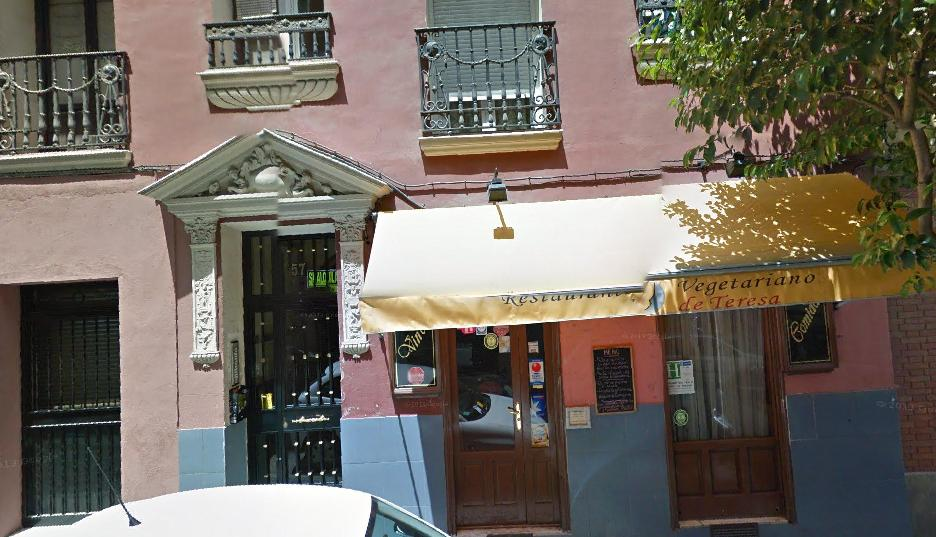
\includegraphics[width=0.49\linewidth]{imgs/cutout_pitch04.jpg}
      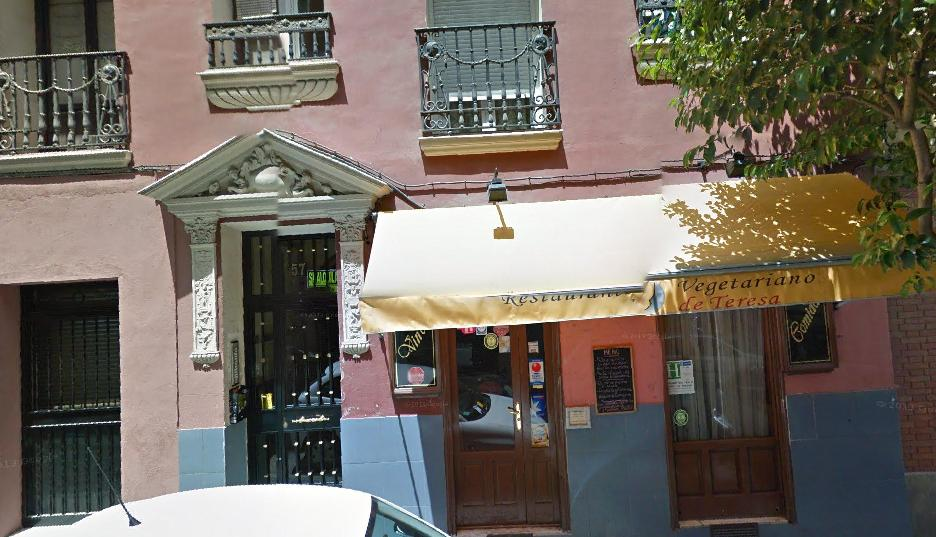
\includegraphics[width=0.49\linewidth]{imgs/cutout_pitch04.jpg}
      \\ \vspace{-3mm} \\
      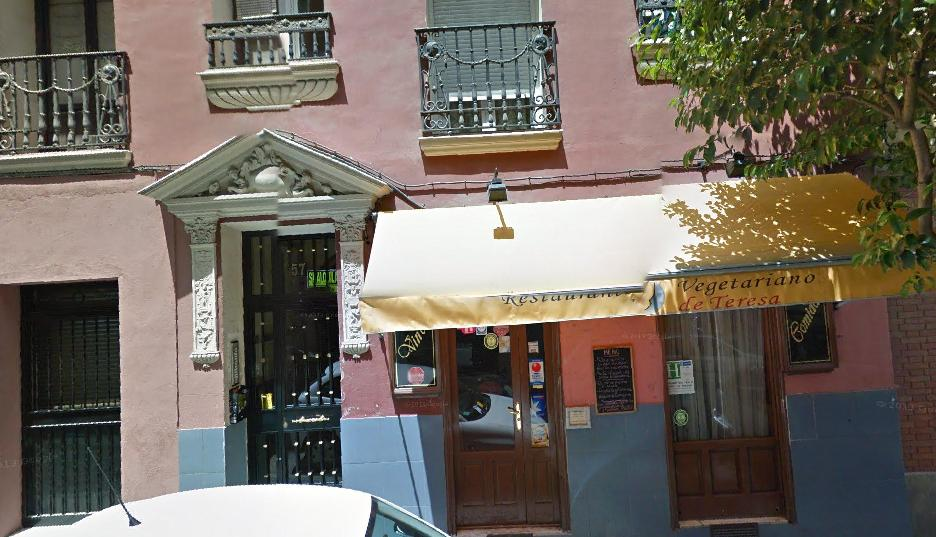
\includegraphics[width=0.49\linewidth]{imgs/cutout_pitch04.jpg}
      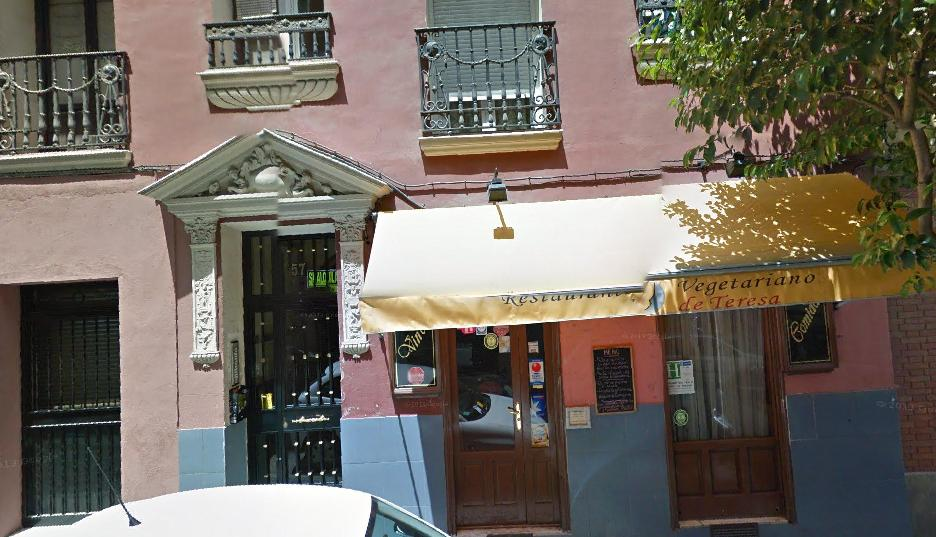
\includegraphics[width=0.49\linewidth]{imgs/cutout_pitch04.jpg}
      \\ \vspace{-3mm} \\
      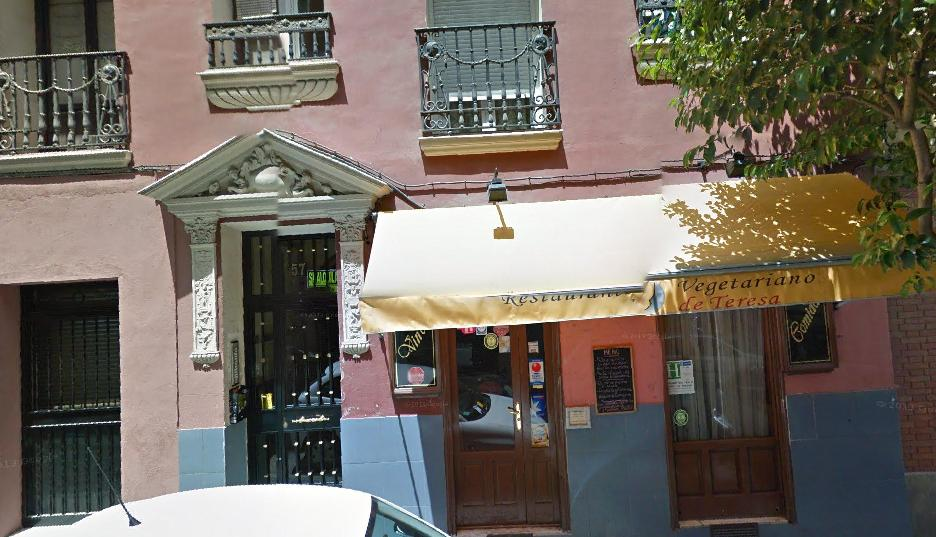
\includegraphics[width=0.49\linewidth]{imgs/cutout_pitch04.jpg}
      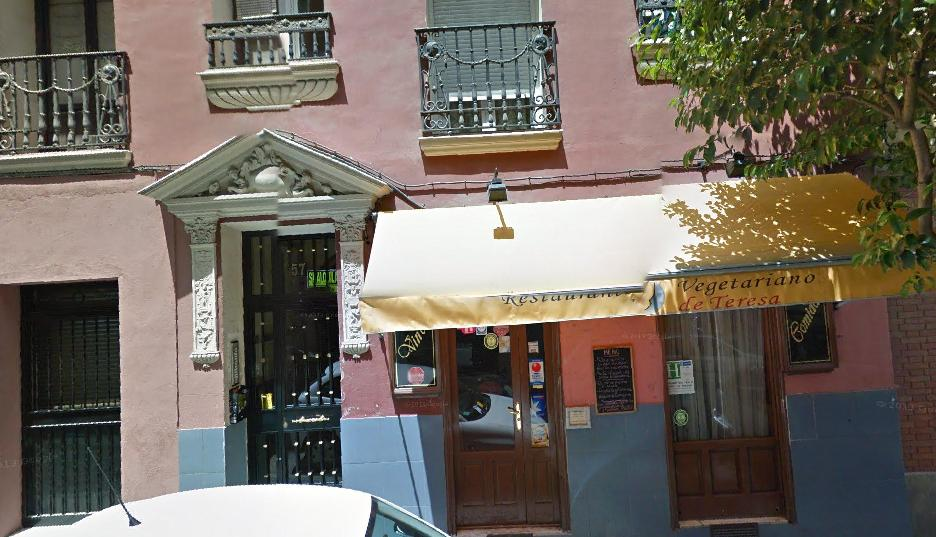
\includegraphics[width=0.49\linewidth]{imgs/cutout_pitch04.jpg}
      \\ \vspace{-3mm} \\
      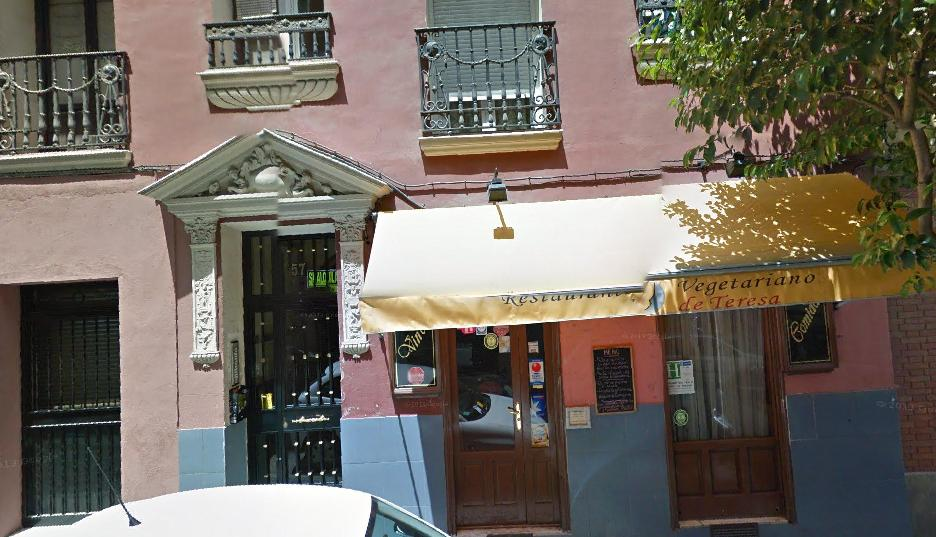
\includegraphics[width=0.49\linewidth]{imgs/cutout_pitch04.jpg}
      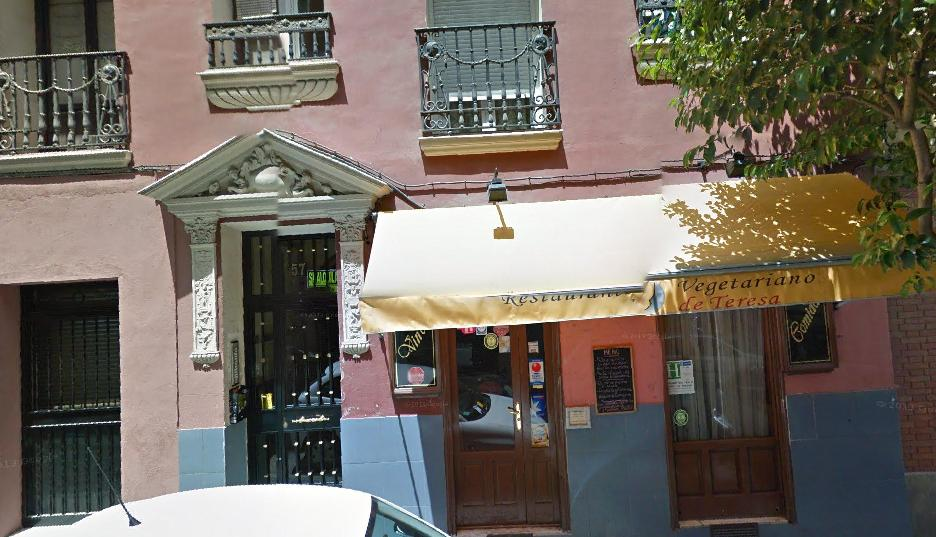
\includegraphics[width=0.49\linewidth]{imgs/cutout_pitch04.jpg}
      \\ \vspace{-3mm} \\
      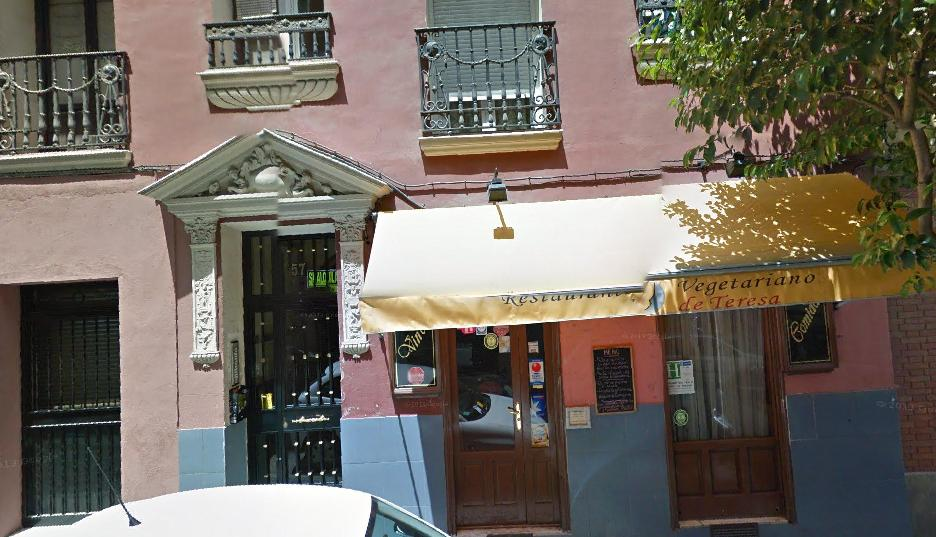
\includegraphics[width=0.49\linewidth]{imgs/cutout_pitch04.jpg}
      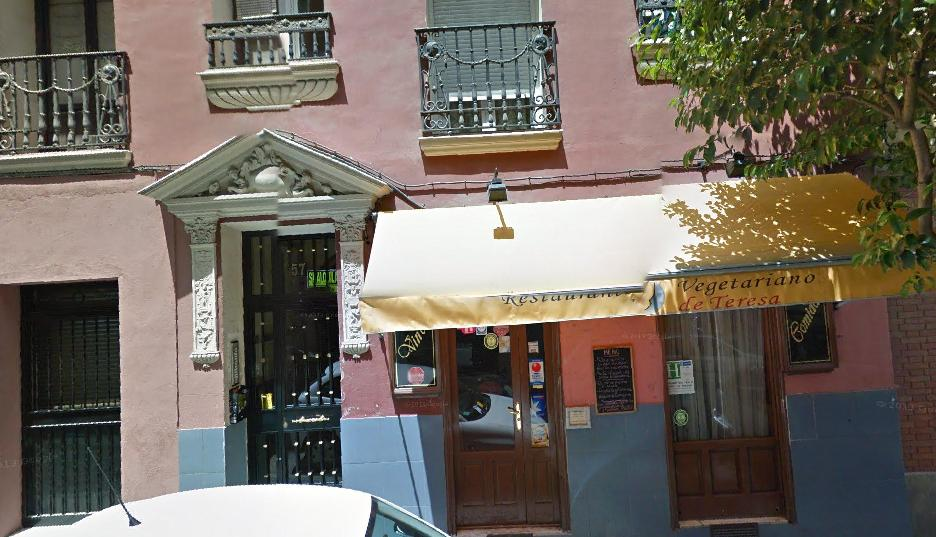
\includegraphics[width=0.49\linewidth]{imgs/cutout_pitch04.jpg}
    \end{minipage}
    \begin{minipage}{0.7\linewidth}
      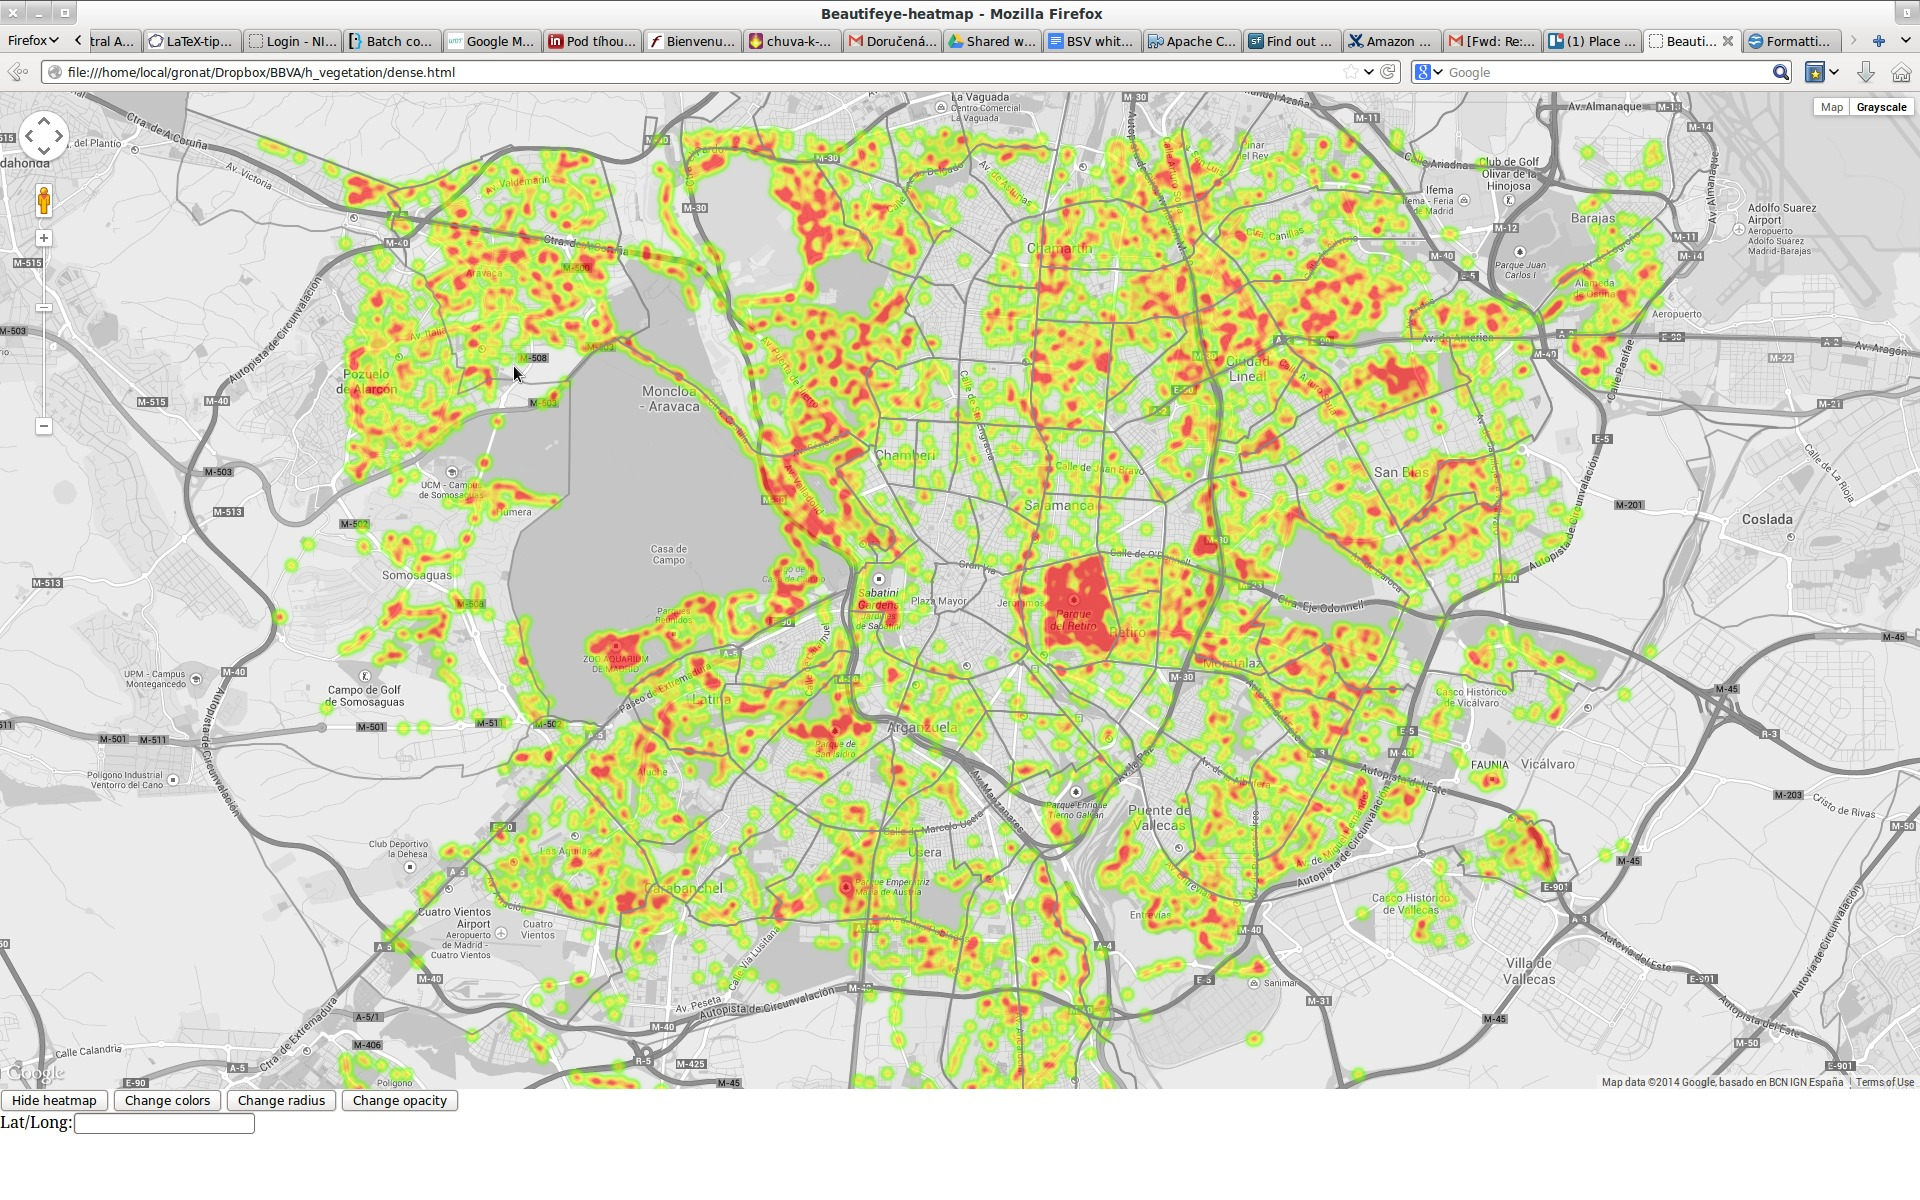
\includegraphics[trim= 350 150 250 150, clip=true, width=\linewidth]{imgs/vege/mapT2.jpg}
    \end{minipage}
  \end{minipage}
  \\
  $\;$ \hspace{30mm} (a) Dense vegetation
  \\
  \\
  \begin{minipage}{\linewidth}
    \begin{minipage}{0.3\linewidth}
      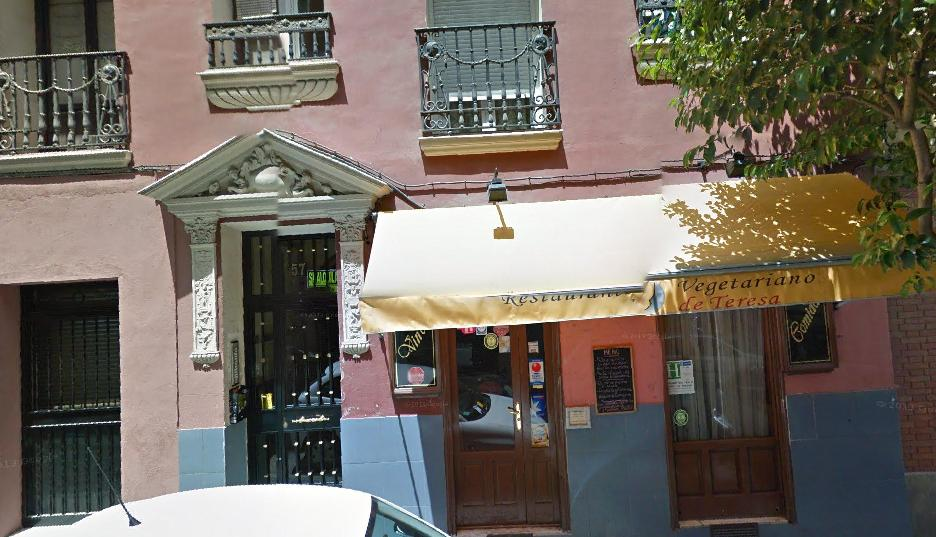
\includegraphics[width=0.49\linewidth]{imgs/cutout_pitch04.jpg}
      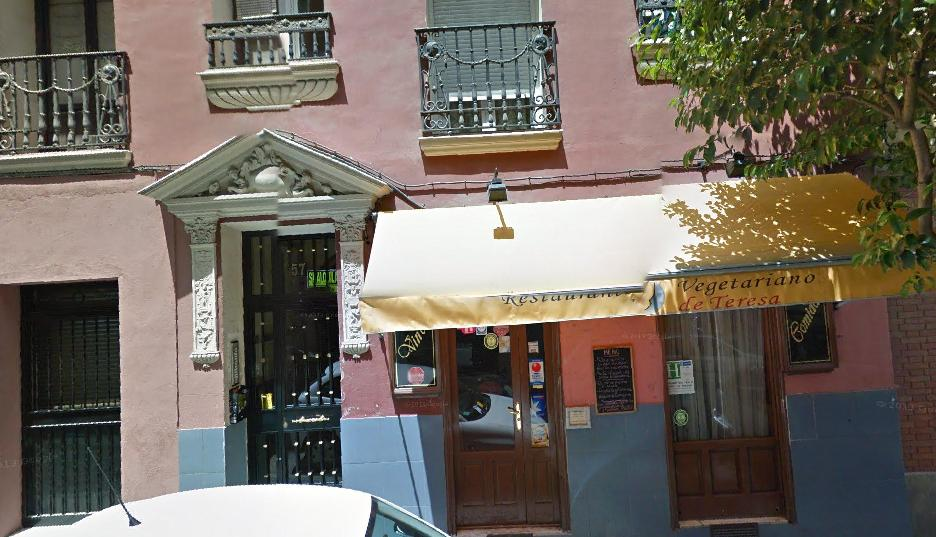
\includegraphics[width=0.49\linewidth]{imgs/cutout_pitch04.jpg}
      \\ \vspace{-3mm} \\
      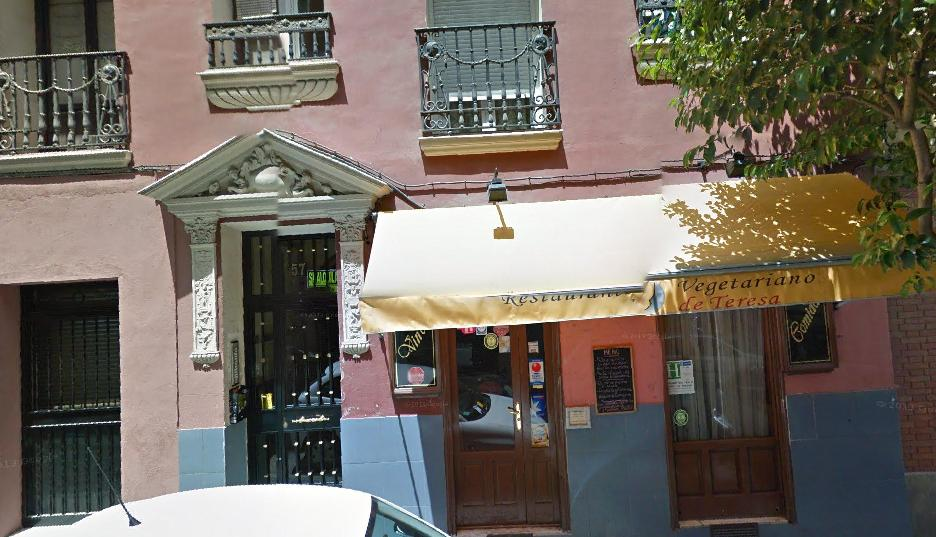
\includegraphics[width=0.49\linewidth]{imgs/cutout_pitch04.jpg}
      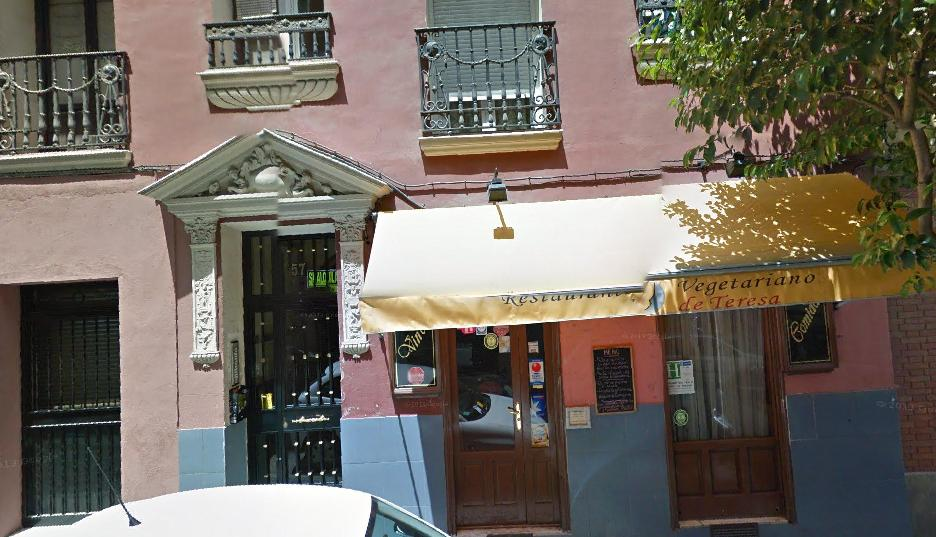
\includegraphics[width=0.49\linewidth]{imgs/cutout_pitch04.jpg}
      \\ \vspace{-3mm} \\
      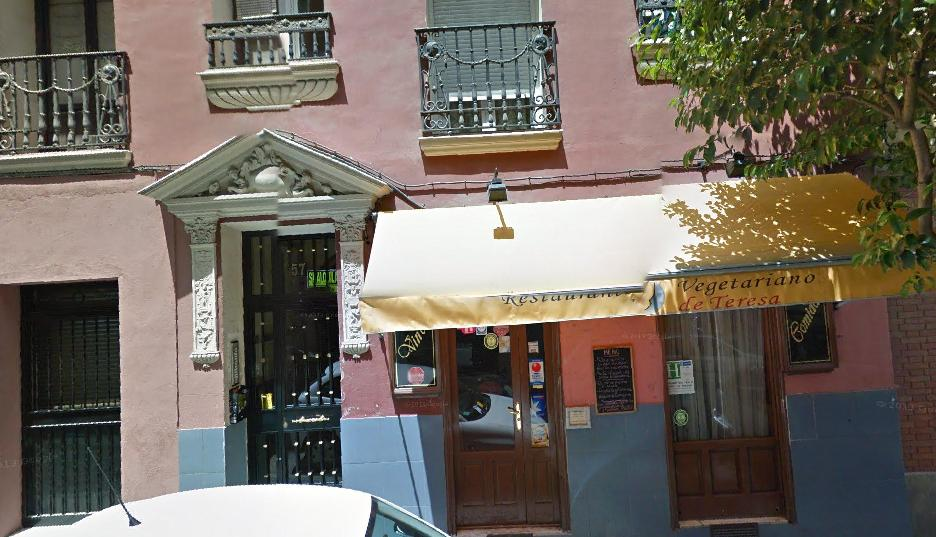
\includegraphics[width=0.49\linewidth]{imgs/cutout_pitch04.jpg}
      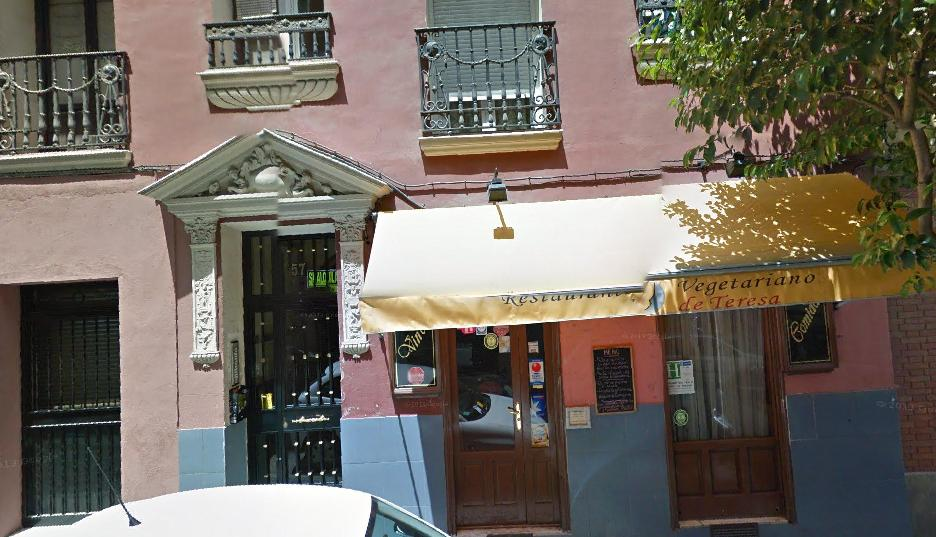
\includegraphics[width=0.49\linewidth]{imgs/cutout_pitch04.jpg}
      \\ \vspace{-3mm} \\
      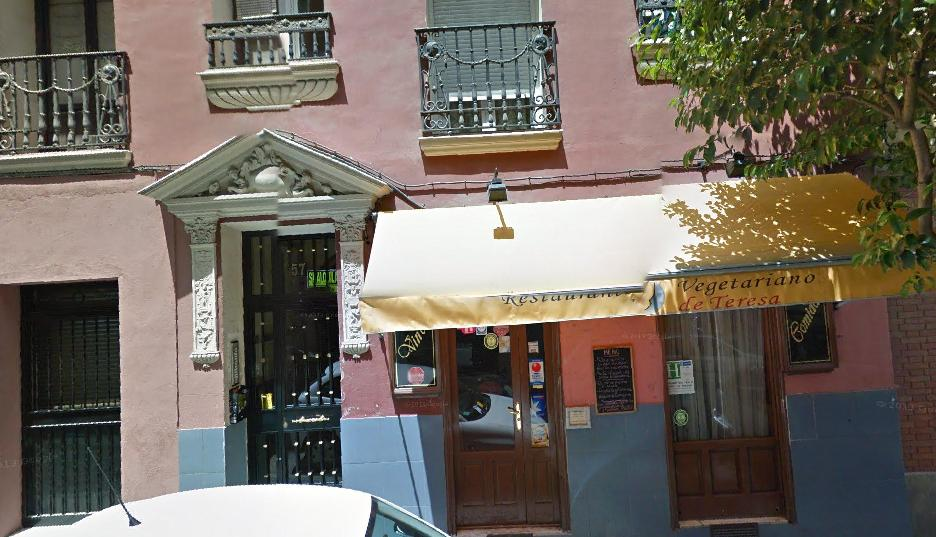
\includegraphics[width=0.49\linewidth]{imgs/cutout_pitch04.jpg}
      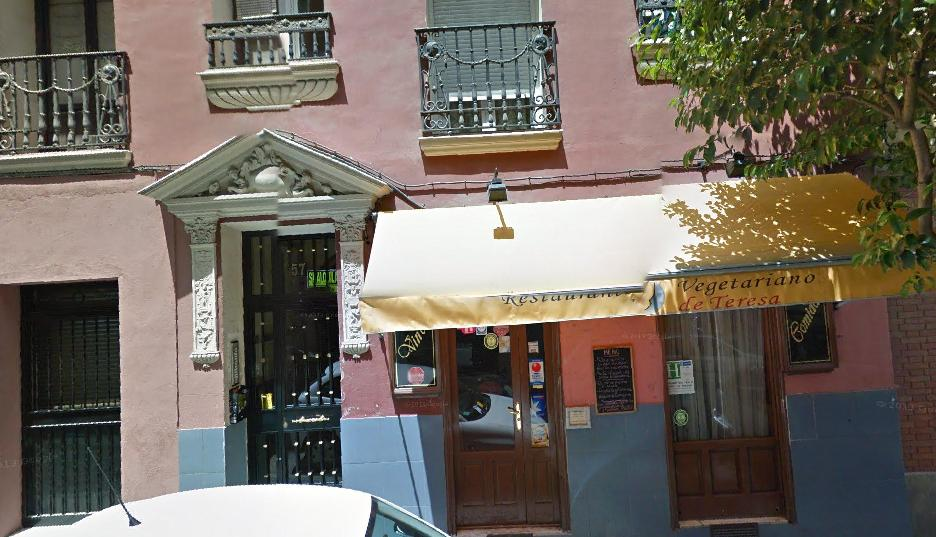
\includegraphics[width=0.49\linewidth]{imgs/cutout_pitch04.jpg}
      \\ \vspace{-3mm} \\
      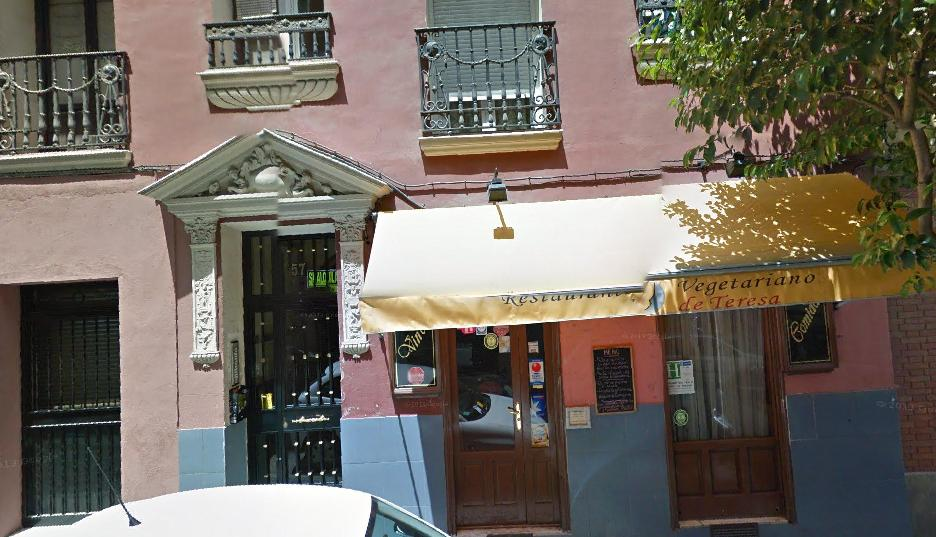
\includegraphics[width=0.49\linewidth]{imgs/cutout_pitch04.jpg}
      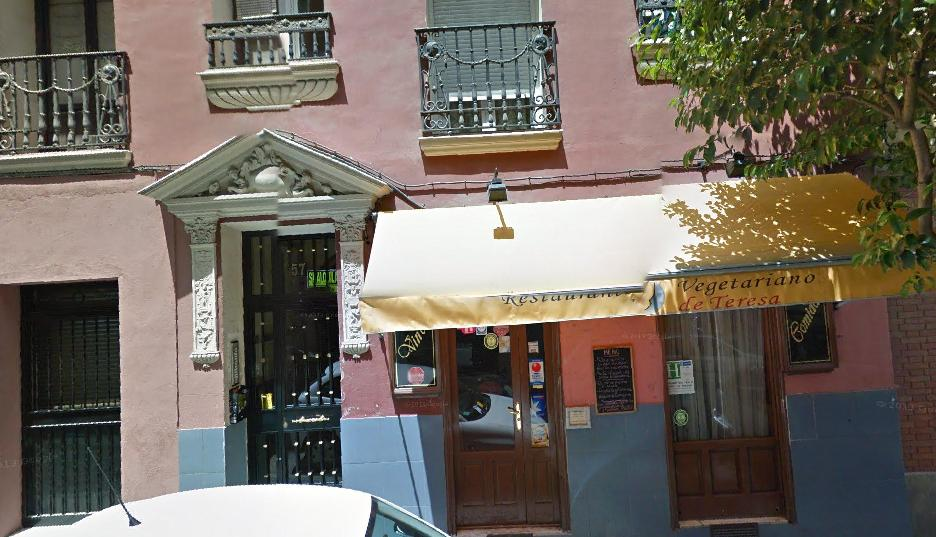
\includegraphics[width=0.49\linewidth]{imgs/cutout_pitch04.jpg}
    \end{minipage}
    \begin{minipage}{0.7\linewidth}
      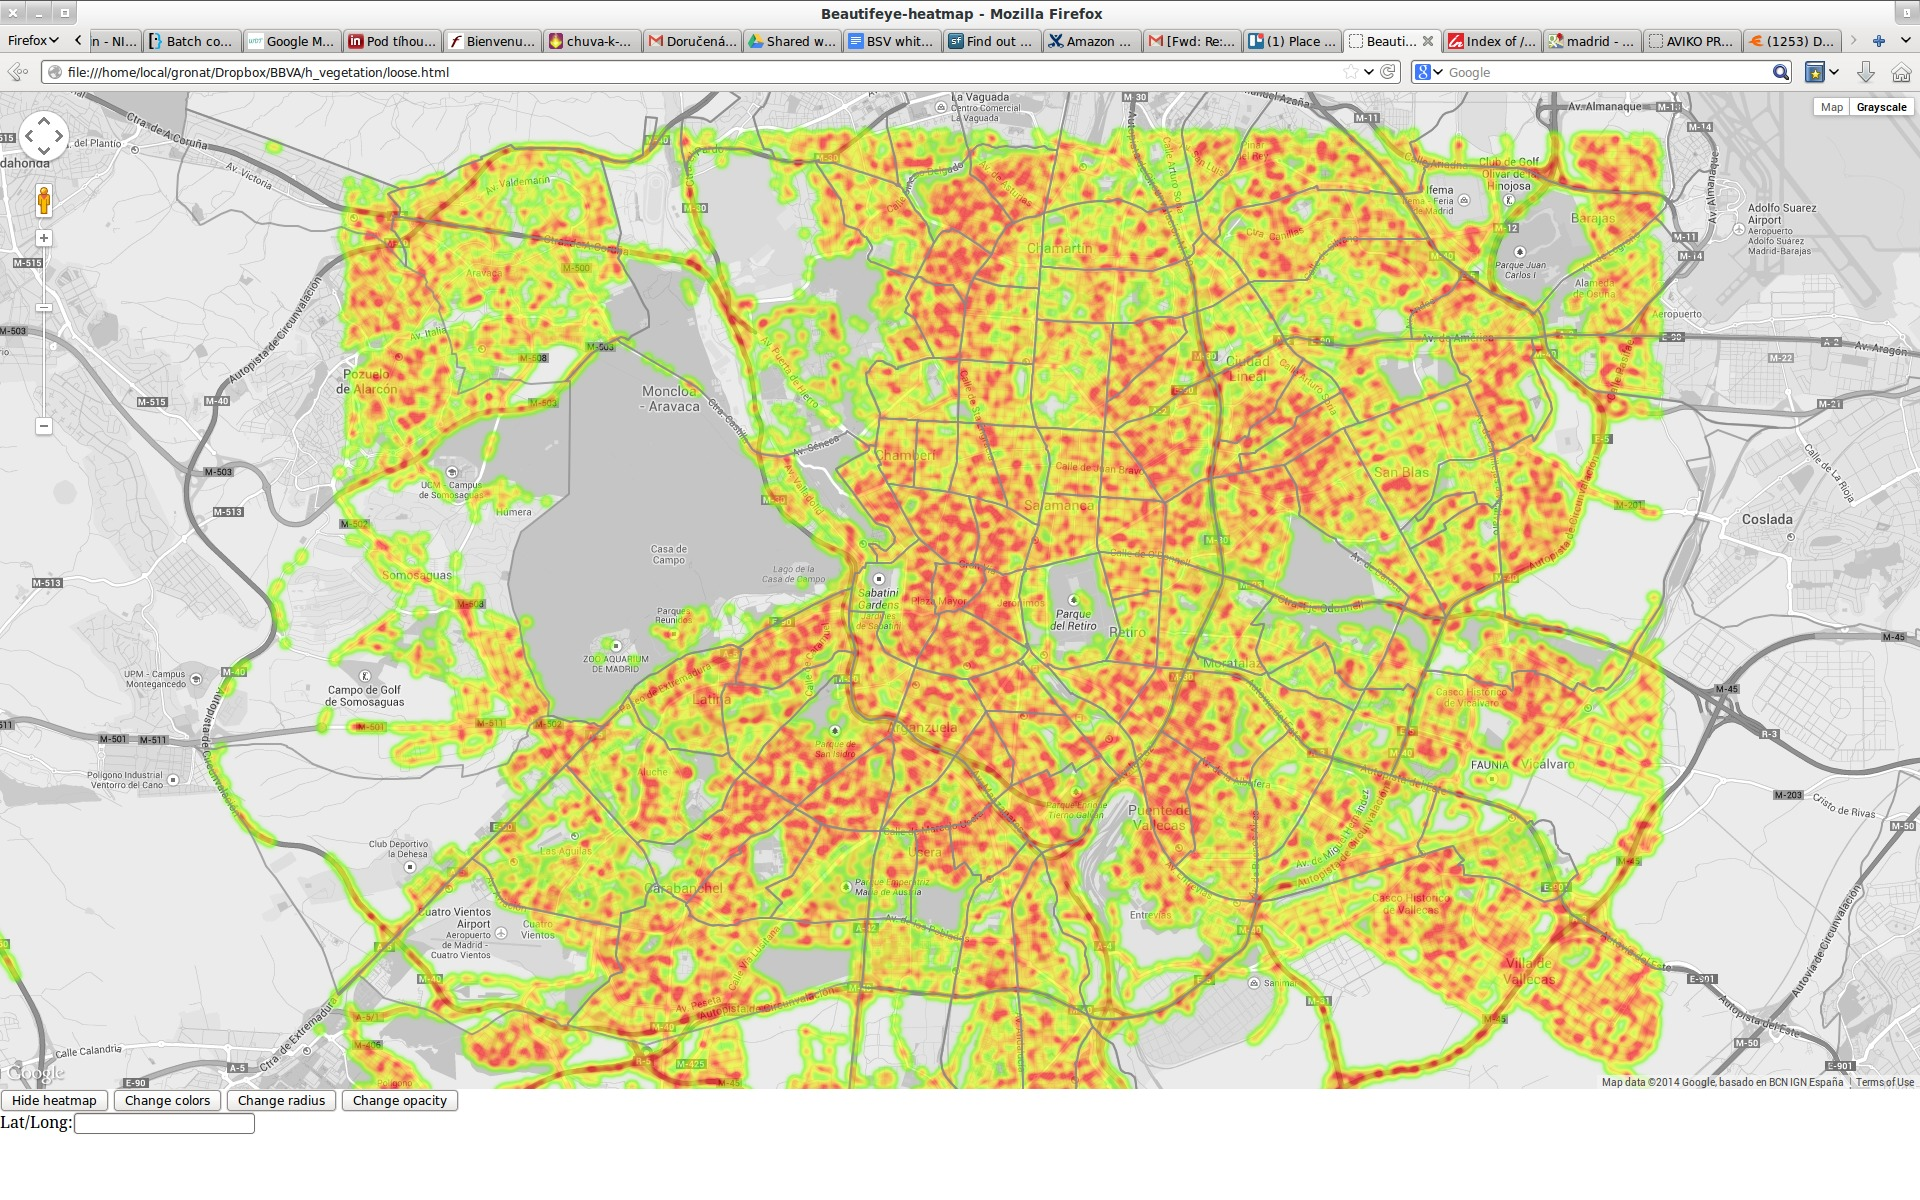
\includegraphics[trim= 350 150 250 150, clip=true, width=\linewidth]{imgs/vege/mapT1.jpg}
    \end{minipage}
  \end{minipage}
  \\
  $\;$\hspace{30mm} (b) Loose vegetation
  \\
  \caption{
    Vegetation: Heatmaps \emph{(right)} showing a density of vegetation across the city of Madrid. Notice a complemetarity of the heatmaps. The \emph{column} shows several top-ranked images by learned predictor.
  }
\end{figure}



\bibliographystyle{splncs}
\bibliography{egbib}
\end{document}
